% IEEE Transactions on Radar Systems -- Regular Paper (IEEEtran journal template).
% R12 (30 Sep 2026): whitened-innovation laws (research/r7c/r12/laws.py, Monte Carlo in verify_laws_output.txt), low-Pfa
% calibration, ANMF baselines, real IPIX targets and certified integration under pulsed interference (PROTOCOL_R12.md,
% frozen at commit 86a7055). Every numeric result is a macro generated from saved outcomes:
% generated/r7_macros.tex, submission_macros.tex, r8_macros.tex, r10_macros.tex, r11_macros.tex and r12_macros.tex
% (../analysis_provenance/make_r12_tables.py). Author biographies/photos: ../final_stage_only/ (final-files stage).
\documentclass[journal]{IEEEtran}
\usepackage[T1]{fontenc}
\usepackage{amsmath,amssymb,amsthm,booktabs,array,graphicx}
\usepackage{cite,xurl,enumitem}
\usepackage[hidelinks]{hyperref}
\graphicspath{{figures/}}
\newtheorem{proposition}{Proposition}
\newtheorem{corollary}{Corollary}
\newtheorem{theorem}{Theorem}
\newcommand{\PP}{\mathbb{P}}
\newcommand{\BelowGOnemEightA}{5}
\newcommand{\BelowGOnemEightB}{0}
\newcommand{\BelowGOnemSixteenA}{4}
\newcommand{\BelowGOnemSixteenB}{0}
\newcommand{\BelowINFourmEightA}{5}
\newcommand{\BelowINFourmEightB}{0}
\newcommand{\BelowINFourmSixteenA}{9}
\newcommand{\BelowINFourmSixteenB}{0}
\newcommand{\BelowINOnemEightA}{0}
\newcommand{\BelowINOnemEightB}{0}
\newcommand{\BelowINOnemSixteenA}{7}
\newcommand{\BelowINOnemSixteenB}{0}
\newcommand{\BelowINTwomEightA}{7}
\newcommand{\BelowINTwomEightB}{0}
\newcommand{\BelowINTwomSixteenA}{4}
\newcommand{\BelowINTwomSixteenB}{0}
\newcommand{\BelowLSmEightA}{2}
\newcommand{\BelowLSmEightB}{0}
\newcommand{\BelowLSmSixteenA}{4}
\newcommand{\BelowLSmSixteenB}{0}
\newcommand{\BelowMLPmEightA}{21}
\newcommand{\BelowMLPmEightB}{0}
\newcommand{\BelowMLPmSixteenA}{21}
\newcommand{\BelowMLPmSixteenB}{0}
\newcommand{\BelowMONmEightA}{4}
\newcommand{\BelowMONmEightB}{0}
\newcommand{\BelowMONmSixteenA}{7}
\newcommand{\BelowMONmSixteenB}{0}
\newcommand{\BelowNAFourGmEightA}{66}
\newcommand{\BelowNAFourGmEightB}{2}
\newcommand{\BelowNAFourGmSixteenA}{29}
\newcommand{\BelowNAFourGmSixteenB}{2}
\newcommand{\BelowNAFourmEightA}{5}
\newcommand{\BelowNAFourmEightB}{0}
\newcommand{\BelowNAFourmSixteenA}{11}
\newcommand{\BelowNAFourmSixteenB}{0}
\newcommand{\BelowNAOneGmEightA}{62}
\newcommand{\BelowNAOneGmEightB}{0}
\newcommand{\BelowNAOneGmSixteenA}{45}
\newcommand{\BelowNAOneGmSixteenB}{2}
\newcommand{\BelowNAOnemEightA}{2}
\newcommand{\BelowNAOnemEightB}{0}
\newcommand{\BelowNAOnemSixteenA}{9}
\newcommand{\BelowNAOnemSixteenB}{0}
\newcommand{\BelowNATwomEightA}{5}
\newcommand{\BelowNATwomEightB}{0}
\newcommand{\BelowNATwomSixteenA}{9}
\newcommand{\BelowNATwomSixteenB}{0}
\newcommand{\BelowRMSmEightA}{29}
\newcommand{\BelowRMSmEightB}{0}
\newcommand{\BelowRMSmSixteenA}{20}
\newcommand{\BelowRMSmSixteenB}{4}
\newcommand{\BelowUmEightA}{25}
\newcommand{\BelowUmEightB}{5}
\newcommand{\BelowUmSixteenA}{21}
\newcommand{\BelowUmSixteenB}{5}
\newcommand{\CFiveCorrA}{0.86}
\newcommand{\CFiveCorrB}{0.96}
\newcommand{\CFiveMaeA}{0.0090}
\newcommand{\CFiveMaeB}{0.0012}
\newcommand{\CFiveNaiveA}{0.0156}
\newcommand{\CFiveNaiveB}{0.0042}
\newcommand{\CleanGOnemEightA}{1.012}
\newcommand{\CleanGOnemEightB}{1.028}
\newcommand{\CleanGOnemSixteenA}{0.997}
\newcommand{\CleanGOnemSixteenB}{0.992}
\newcommand{\CleanINFourmEightA}{0.848}
\newcommand{\CleanINFourmEightB}{0.933}
\newcommand{\CleanINFourmSixteenA}{0.802}
\newcommand{\CleanINFourmSixteenB}{0.820}
\newcommand{\CleanINOnemEightA}{1.000}
\newcommand{\CleanINOnemEightB}{1.000}
\newcommand{\CleanINOnemSixteenA}{1.000}
\newcommand{\CleanINOnemSixteenB}{1.000}
\newcommand{\CleanINTwomEightA}{0.878}
\newcommand{\CleanINTwomEightB}{0.932}
\newcommand{\CleanINTwomSixteenA}{0.865}
\newcommand{\CleanINTwomSixteenB}{0.873}
\newcommand{\CleanLSmEightA}{0.859}
\newcommand{\CleanLSmEightB}{0.967}
\newcommand{\CleanLSmSixteenA}{0.871}
\newcommand{\CleanLSmSixteenB}{1.018}
\newcommand{\CleanMLPmEightA}{1.378}
\newcommand{\CleanMLPmEightB}{1.862}
\newcommand{\CleanMLPmSixteenA}{1.390}
\newcommand{\CleanMLPmSixteenB}{1.740}
\newcommand{\CleanMONmEightA}{0.953}
\newcommand{\CleanMONmEightB}{0.952}
\newcommand{\CleanMONmSixteenA}{0.980}
\newcommand{\CleanMONmSixteenB}{1.002}
\newcommand{\CleanNAFourGmEightA}{0.666}
\newcommand{\CleanNAFourGmEightB}{0.626}
\newcommand{\CleanNAFourGmSixteenA}{0.682}
\newcommand{\CleanNAFourGmSixteenB}{0.654}
\newcommand{\CleanNAFourmEightA}{0.706}
\newcommand{\CleanNAFourmEightB}{0.695}
\newcommand{\CleanNAFourmSixteenA}{0.709}
\newcommand{\CleanNAFourmSixteenB}{0.704}
\newcommand{\CleanNAOneGmEightA}{0.927}
\newcommand{\CleanNAOneGmEightB}{0.873}
\newcommand{\CleanNAOneGmSixteenA}{0.952}
\newcommand{\CleanNAOneGmSixteenB}{0.913}
\newcommand{\CleanNAOnemEightA}{0.985}
\newcommand{\CleanNAOnemEightB}{0.982}
\newcommand{\CleanNAOnemSixteenA}{0.989}
\newcommand{\CleanNAOnemSixteenB}{0.984}
\newcommand{\CleanNATwomEightA}{0.738}
\newcommand{\CleanNATwomEightB}{0.731}
\newcommand{\CleanNATwomSixteenA}{0.739}
\newcommand{\CleanNATwomSixteenB}{0.738}
\newcommand{\CleanRMSmEightA}{1.480}
\newcommand{\CleanRMSmEightB}{1.930}
\newcommand{\CleanRMSmSixteenA}{1.404}
\newcommand{\CleanRMSmSixteenB}{1.729}
\newcommand{\CleanUmEightA}{1.065}
\newcommand{\CleanUmEightB}{1.660}
\newcommand{\CleanUmSixteenA}{1.073}
\newcommand{\CleanUmSixteenB}{1.700}
\newcommand{\CovGOnemEightA}{0.903}
\newcommand{\CovGOnemEightB}{0.991}
\newcommand{\CovGOnemSixteenA}{0.900}
\newcommand{\CovGOnemSixteenB}{0.990}
\newcommand{\CovINFourmEightA}{0.901}
\newcommand{\CovINFourmEightB}{0.991}
\newcommand{\CovINFourmSixteenA}{0.901}
\newcommand{\CovINFourmSixteenB}{0.990}
\newcommand{\CovINOnemEightA}{0.902}
\newcommand{\CovINOnemEightB}{0.991}
\newcommand{\CovINOnemSixteenA}{0.901}
\newcommand{\CovINOnemSixteenB}{0.990}
\newcommand{\CovINTwomEightA}{0.901}
\newcommand{\CovINTwomEightB}{0.991}
\newcommand{\CovINTwomSixteenA}{0.901}
\newcommand{\CovINTwomSixteenB}{0.990}
\newcommand{\CovLSmEightA}{0.899}
\newcommand{\CovLSmEightB}{0.990}
\newcommand{\CovLSmSixteenA}{0.900}
\newcommand{\CovLSmSixteenB}{0.991}
\newcommand{\CovMLPmEightA}{0.898}
\newcommand{\CovMLPmEightB}{0.990}
\newcommand{\CovMLPmSixteenA}{0.901}
\newcommand{\CovMLPmSixteenB}{0.990}
\newcommand{\CovMONmEightA}{0.903}
\newcommand{\CovMONmEightB}{0.993}
\newcommand{\CovMONmSixteenA}{0.904}
\newcommand{\CovMONmSixteenB}{0.992}
\newcommand{\CovMinGOnemEightA}{0.860}
\newcommand{\CovMinGOnemEightB}{0.978}
\newcommand{\CovMinGOnemSixteenA}{0.845}
\newcommand{\CovMinGOnemSixteenB}{0.979}
\newcommand{\CovMinINFourmEightA}{0.873}
\newcommand{\CovMinINFourmEightB}{0.982}
\newcommand{\CovMinINFourmSixteenA}{0.869}
\newcommand{\CovMinINFourmSixteenB}{0.978}
\newcommand{\CovMinINOnemEightA}{0.880}
\newcommand{\CovMinINOnemEightB}{0.980}
\newcommand{\CovMinINOnemSixteenA}{0.864}
\newcommand{\CovMinINOnemSixteenB}{0.973}
\newcommand{\CovMinINTwomEightA}{0.862}
\newcommand{\CovMinINTwomEightB}{0.983}
\newcommand{\CovMinINTwomSixteenA}{0.871}
\newcommand{\CovMinINTwomSixteenB}{0.982}
\newcommand{\CovMinLSmEightA}{0.878}
\newcommand{\CovMinLSmEightB}{0.982}
\newcommand{\CovMinLSmSixteenA}{0.866}
\newcommand{\CovMinLSmSixteenB}{0.981}
\newcommand{\CovMinMLPmEightA}{0.854}
\newcommand{\CovMinMLPmEightB}{0.979}
\newcommand{\CovMinMLPmSixteenA}{0.850}
\newcommand{\CovMinMLPmSixteenB}{0.977}
\newcommand{\CovMinMONmEightA}{0.873}
\newcommand{\CovMinMONmEightB}{0.982}
\newcommand{\CovMinMONmSixteenA}{0.862}
\newcommand{\CovMinMONmSixteenB}{0.984}
\newcommand{\CovMinNAFourGmEightA}{0.806}
\newcommand{\CovMinNAFourGmEightB}{0.968}
\newcommand{\CovMinNAFourGmSixteenA}{0.811}
\newcommand{\CovMinNAFourGmSixteenB}{0.964}
\newcommand{\CovMinNAFourmEightA}{0.873}
\newcommand{\CovMinNAFourmEightB}{0.983}
\newcommand{\CovMinNAFourmSixteenA}{0.853}
\newcommand{\CovMinNAFourmSixteenB}{0.980}
\newcommand{\CovMinNAOneGmEightA}{0.805}
\newcommand{\CovMinNAOneGmEightB}{0.972}
\newcommand{\CovMinNAOneGmSixteenA}{0.812}
\newcommand{\CovMinNAOneGmSixteenB}{0.968}
\newcommand{\CovMinNAOnemEightA}{0.877}
\newcommand{\CovMinNAOnemEightB}{0.980}
\newcommand{\CovMinNAOnemSixteenA}{0.855}
\newcommand{\CovMinNAOnemSixteenB}{0.975}
\newcommand{\CovMinNATwomEightA}{0.866}
\newcommand{\CovMinNATwomEightB}{0.980}
\newcommand{\CovMinNATwomSixteenA}{0.861}
\newcommand{\CovMinNATwomSixteenB}{0.978}
\newcommand{\CovMinRMSmEightA}{0.861}
\newcommand{\CovMinRMSmEightB}{0.979}
\newcommand{\CovMinRMSmSixteenA}{0.845}
\newcommand{\CovMinRMSmSixteenB}{0.963}
\newcommand{\CovMinUmEightA}{0.781}
\newcommand{\CovMinUmEightB}{0.949}
\newcommand{\CovMinUmSixteenA}{0.801}
\newcommand{\CovMinUmSixteenB}{0.967}
\newcommand{\CovNAFourGmEightA}{0.873}
\newcommand{\CovNAFourGmEightB}{0.982}
\newcommand{\CovNAFourGmSixteenA}{0.885}
\newcommand{\CovNAFourGmSixteenB}{0.985}
\newcommand{\CovNAFourmEightA}{0.900}
\newcommand{\CovNAFourmEightB}{0.990}
\newcommand{\CovNAFourmSixteenA}{0.902}
\newcommand{\CovNAFourmSixteenB}{0.991}
\newcommand{\CovNAOneGmEightA}{0.874}
\newcommand{\CovNAOneGmEightB}{0.981}
\newcommand{\CovNAOneGmSixteenA}{0.882}
\newcommand{\CovNAOneGmSixteenB}{0.984}
\newcommand{\CovNAOnemEightA}{0.901}
\newcommand{\CovNAOnemEightB}{0.991}
\newcommand{\CovNAOnemSixteenA}{0.901}
\newcommand{\CovNAOnemSixteenB}{0.990}
\newcommand{\CovNATwomEightA}{0.900}
\newcommand{\CovNATwomEightB}{0.991}
\newcommand{\CovNATwomSixteenA}{0.901}
\newcommand{\CovNATwomSixteenB}{0.991}
\newcommand{\CovRMSmEightA}{0.899}
\newcommand{\CovRMSmEightB}{0.991}
\newcommand{\CovRMSmSixteenA}{0.899}
\newcommand{\CovRMSmSixteenB}{0.989}
\newcommand{\CovUmEightA}{0.899}
\newcommand{\CovUmEightB}{0.989}
\newcommand{\CovUmSixteenA}{0.899}
\newcommand{\CovUmSixteenB}{0.989}
\newcommand{\CurveHighGOnemEightA}{0.918}
\newcommand{\CurveHighGOnemEightB}{0.995}
\newcommand{\CurveHighGOnemSixteenA}{0.908}
\newcommand{\CurveHighGOnemSixteenB}{0.993}
\newcommand{\CurveHighINFourmEightA}{0.902}
\newcommand{\CurveHighINFourmEightB}{0.992}
\newcommand{\CurveHighINFourmSixteenA}{0.903}
\newcommand{\CurveHighINFourmSixteenB}{0.991}
\newcommand{\CurveHighINOnemEightA}{0.917}
\newcommand{\CurveHighINOnemEightB}{0.994}
\newcommand{\CurveHighINOnemSixteenA}{0.908}
\newcommand{\CurveHighINOnemSixteenB}{0.993}
\newcommand{\CurveHighINTwomEightA}{0.902}
\newcommand{\CurveHighINTwomEightB}{0.993}
\newcommand{\CurveHighINTwomSixteenA}{0.902}
\newcommand{\CurveHighINTwomSixteenB}{0.990}
\newcommand{\CurveHighLSmEightA}{0.883}
\newcommand{\CurveHighLSmEightB}{0.986}
\newcommand{\CurveHighLSmSixteenA}{0.890}
\newcommand{\CurveHighLSmSixteenB}{0.987}
\newcommand{\CurveHighMLPmEightA}{0.948}
\newcommand{\CurveHighMLPmEightB}{0.997}
\newcommand{\CurveHighMLPmSixteenA}{0.950}
\newcommand{\CurveHighMLPmSixteenB}{0.995}
\newcommand{\CurveHighMONmEightA}{0.878}
\newcommand{\CurveHighMONmEightB}{0.988}
\newcommand{\CurveHighMONmSixteenA}{0.887}
\newcommand{\CurveHighMONmSixteenB}{0.989}
\newcommand{\CurveHighNAFourGmEightA}{0.863}
\newcommand{\CurveHighNAFourGmEightB}{0.978}
\newcommand{\CurveHighNAFourGmSixteenA}{0.880}
\newcommand{\CurveHighNAFourGmSixteenB}{0.981}
\newcommand{\CurveHighNAFourmEightA}{0.890}
\newcommand{\CurveHighNAFourmEightB}{0.988}
\newcommand{\CurveHighNAFourmSixteenA}{0.898}
\newcommand{\CurveHighNAFourmSixteenB}{0.988}
\newcommand{\CurveHighNAOneGmEightA}{0.887}
\newcommand{\CurveHighNAOneGmEightB}{0.986}
\newcommand{\CurveHighNAOneGmSixteenA}{0.894}
\newcommand{\CurveHighNAOneGmSixteenB}{0.987}
\newcommand{\CurveHighNAOnemEightA}{0.915}
\newcommand{\CurveHighNAOnemEightB}{0.993}
\newcommand{\CurveHighNAOnemSixteenA}{0.911}
\newcommand{\CurveHighNAOnemSixteenB}{0.992}
\newcommand{\CurveHighNATwomEightA}{0.898}
\newcommand{\CurveHighNATwomEightB}{0.991}
\newcommand{\CurveHighNATwomSixteenA}{0.905}
\newcommand{\CurveHighNATwomSixteenB}{0.989}
\newcommand{\CurveHighRMSmEightA}{0.951}
\newcommand{\CurveHighRMSmEightB}{0.997}
\newcommand{\CurveHighRMSmSixteenA}{0.957}
\newcommand{\CurveHighRMSmSixteenB}{0.997}
\newcommand{\CurveHighUmEightA}{0.741}
\newcommand{\CurveHighUmEightB}{0.954}
\newcommand{\CurveHighUmSixteenA}{0.744}
\newcommand{\CurveHighUmSixteenB}{0.953}
\newcommand{\CurveLowGOnemEightA}{0.889}
\newcommand{\CurveLowGOnemEightB}{0.989}
\newcommand{\CurveLowGOnemSixteenA}{0.894}
\newcommand{\CurveLowGOnemSixteenB}{0.988}
\newcommand{\CurveLowINFourmEightA}{0.900}
\newcommand{\CurveLowINFourmEightB}{0.990}
\newcommand{\CurveLowINFourmSixteenA}{0.900}
\newcommand{\CurveLowINFourmSixteenB}{0.989}
\newcommand{\CurveLowINOnemEightA}{0.889}
\newcommand{\CurveLowINOnemEightB}{0.988}
\newcommand{\CurveLowINOnemSixteenA}{0.896}
\newcommand{\CurveLowINOnemSixteenB}{0.988}
\newcommand{\CurveLowINTwomEightA}{0.902}
\newcommand{\CurveLowINTwomEightB}{0.991}
\newcommand{\CurveLowINTwomSixteenA}{0.899}
\newcommand{\CurveLowINTwomSixteenB}{0.989}
\newcommand{\CurveLowLSmEightA}{0.909}
\newcommand{\CurveLowLSmEightB}{0.992}
\newcommand{\CurveLowLSmSixteenA}{0.908}
\newcommand{\CurveLowLSmSixteenB}{0.992}
\newcommand{\CurveLowMLPmEightA}{0.824}
\newcommand{\CurveLowMLPmEightB}{0.980}
\newcommand{\CurveLowMLPmSixteenA}{0.818}
\newcommand{\CurveLowMLPmSixteenB}{0.977}
\newcommand{\CurveLowMONmEightA}{0.927}
\newcommand{\CurveLowMONmEightB}{0.996}
\newcommand{\CurveLowMONmSixteenA}{0.921}
\newcommand{\CurveLowMONmSixteenB}{0.995}
\newcommand{\CurveLowNAFourGmEightA}{0.893}
\newcommand{\CurveLowNAFourGmEightB}{0.986}
\newcommand{\CurveLowNAFourGmSixteenA}{0.899}
\newcommand{\CurveLowNAFourGmSixteenB}{0.987}
\newcommand{\CurveLowNAFourmEightA}{0.918}
\newcommand{\CurveLowNAFourmEightB}{0.993}
\newcommand{\CurveLowNAFourmSixteenA}{0.916}
\newcommand{\CurveLowNAFourmSixteenB}{0.993}
\newcommand{\CurveLowNAOneGmEightA}{0.865}
\newcommand{\CurveLowNAOneGmEightB}{0.978}
\newcommand{\CurveLowNAOneGmSixteenA}{0.877}
\newcommand{\CurveLowNAOneGmSixteenB}{0.981}
\newcommand{\CurveLowNAOnemEightA}{0.895}
\newcommand{\CurveLowNAOnemEightB}{0.989}
\newcommand{\CurveLowNAOnemSixteenA}{0.898}
\newcommand{\CurveLowNAOnemSixteenB}{0.988}
\newcommand{\CurveLowNATwomEightA}{0.910}
\newcommand{\CurveLowNATwomEightB}{0.991}
\newcommand{\CurveLowNATwomSixteenA}{0.907}
\newcommand{\CurveLowNATwomSixteenB}{0.991}
\newcommand{\CurveLowRMSmEightA}{0.820}
\newcommand{\CurveLowRMSmEightB}{0.981}
\newcommand{\CurveLowRMSmSixteenA}{0.812}
\newcommand{\CurveLowRMSmSixteenB}{0.974}
\newcommand{\CurveLowUmEightA}{0.982}
\newcommand{\CurveLowUmEightB}{0.999}
\newcommand{\CurveLowUmSixteenA}{0.978}
\newcommand{\CurveLowUmSixteenB}{0.999}
\newcommand{\HoCovGOne}{0.945}
\newcommand{\HoCovINFour}{0.906}
\newcommand{\HoCovINOne}{0.910}
\newcommand{\HoCovINTwo}{0.906}
\newcommand{\HoCovLS}{0.919}
\newcommand{\HoCovMLP}{0.903}
\newcommand{\HoCovMON}{0.896}
\newcommand{\HoCovNAFour}{0.893}
\newcommand{\HoCovNAFourG}{0.856}
\newcommand{\HoCovNAOne}{0.903}
\newcommand{\HoCovNATwo}{0.895}
\newcommand{\HoCovRMS}{0.887}
\newcommand{\HoCovU}{0.859}
\newcommand{\HoMonInf}{infinite}
\newcommand{\HoRatioGOne}{1.104}
\newcommand{\HoRatioINFour}{0.515}
\newcommand{\HoRatioINOne}{1.000}
\newcommand{\HoRatioINTwo}{0.572}
\newcommand{\HoRatioLS}{0.662}
\newcommand{\HoRatioMLP}{2.158}
\newcommand{\HoRatioMON}{0.981}
\newcommand{\HoRatioNAFour}{0.498}
\newcommand{\HoRatioNAFourG}{0.472}
\newcommand{\HoRatioNAOne}{0.921}
\newcommand{\HoRatioNATwo}{0.533}
\newcommand{\HoRatioRMS}{1.243}
\newcommand{\HoRatioU}{1.161}
\newcommand{\MaxdevGOnemEightA}{0.038}
\newcommand{\MaxdevGOnemEightB}{0.011}
\newcommand{\MaxdevGOnemSixteenA}{0.034}
\newcommand{\MaxdevGOnemSixteenB}{0.011}
\newcommand{\MaxdevINFourmEightA}{0.031}
\newcommand{\MaxdevINFourmEightB}{0.010}
\newcommand{\MaxdevINFourmSixteenA}{0.032}
\newcommand{\MaxdevINFourmSixteenB}{0.011}
\newcommand{\MaxdevINOneWFiveTwelve}{0.035}
\newcommand{\MaxdevINOneWTwentyFortyEight}{0.033}
\newcommand{\MaxdevINOnemEightA}{0.037}
\newcommand{\MaxdevINOnemEightB}{0.011}
\newcommand{\MaxdevINOnemSixteenA}{0.036}
\newcommand{\MaxdevINOnemSixteenB}{0.011}
\newcommand{\MaxdevINTwomEightA}{0.035}
\newcommand{\MaxdevINTwomEightB}{0.010}
\newcommand{\MaxdevINTwomSixteenA}{0.034}
\newcommand{\MaxdevINTwomSixteenB}{0.010}
\newcommand{\MaxdevLSmEightA}{0.039}
\newcommand{\MaxdevLSmEightB}{0.012}
\newcommand{\MaxdevLSmSixteenA}{0.039}
\newcommand{\MaxdevLSmSixteenB}{0.012}
\newcommand{\MaxdevMLPWFiveTwelve}{0.103}
\newcommand{\MaxdevMLPWTwentyFortyEight}{0.080}
\newcommand{\MaxdevMLPmEightA}{0.092}
\newcommand{\MaxdevMLPmEightB}{0.015}
\newcommand{\MaxdevMLPmSixteenA}{0.096}
\newcommand{\MaxdevMLPmSixteenB}{0.019}
\newcommand{\MaxdevMONWFiveTwelve}{0.042}
\newcommand{\MaxdevMONWTwentyFortyEight}{0.039}
\newcommand{\MaxdevMONmEightA}{0.043}
\newcommand{\MaxdevMONmEightB}{0.010}
\newcommand{\MaxdevMONmSixteenA}{0.043}
\newcommand{\MaxdevMONmSixteenB}{0.011}
\newcommand{\MaxdevNAFourGmEightA}{0.063}
\newcommand{\MaxdevNAFourGmEightB}{0.020}
\newcommand{\MaxdevNAFourGmSixteenA}{0.049}
\newcommand{\MaxdevNAFourGmSixteenB}{0.016}
\newcommand{\MaxdevNAFourWFiveTwelve}{0.043}
\newcommand{\MaxdevNAFourWTwentyFortyEight}{0.043}
\newcommand{\MaxdevNAFourmEightA}{0.043}
\newcommand{\MaxdevNAFourmEightB}{0.010}
\newcommand{\MaxdevNAFourmSixteenA}{0.043}
\newcommand{\MaxdevNAFourmSixteenB}{0.011}
\newcommand{\MaxdevNAOneGmEightA}{0.062}
\newcommand{\MaxdevNAOneGmEightB}{0.021}
\newcommand{\MaxdevNAOneGmSixteenA}{0.051}
\newcommand{\MaxdevNAOneGmSixteenB}{0.017}
\newcommand{\MaxdevNAOnemEightA}{0.043}
\newcommand{\MaxdevNAOnemEightB}{0.012}
\newcommand{\MaxdevNAOnemSixteenA}{0.042}
\newcommand{\MaxdevNAOnemSixteenB}{0.011}
\newcommand{\MaxdevNATwomEightA}{0.042}
\newcommand{\MaxdevNATwomEightB}{0.011}
\newcommand{\MaxdevNATwomSixteenA}{0.044}
\newcommand{\MaxdevNATwomSixteenB}{0.011}
\newcommand{\MaxdevRMSWFiveTwelve}{0.110}
\newcommand{\MaxdevRMSWTwentyFortyEight}{0.086}
\newcommand{\MaxdevRMSmEightA}{0.096}
\newcommand{\MaxdevRMSmEightB}{0.015}
\newcommand{\MaxdevRMSmSixteenA}{0.103}
\newcommand{\MaxdevRMSmSixteenB}{0.021}
\newcommand{\MaxdevUWFiveTwelve}{0.181}
\newcommand{\MaxdevUWTwentyFortyEight}{0.141}
\newcommand{\MaxdevUmEightA}{0.170}
\newcommand{\MaxdevUmEightB}{0.038}
\newcommand{\MaxdevUmSixteenA}{0.165}
\newcommand{\MaxdevUmSixteenB}{0.039}
\newcommand{\NCleanConf}{39}
\newcommand{\NNoisyConf}{17}
\newcommand{\NUnitsConf}{56}
\newcommand{\NoisyGOnemEightA}{0.979}
\newcommand{\NoisyGOnemEightB}{0.949}
\newcommand{\NoisyGOnemSixteenA}{0.990}
\newcommand{\NoisyGOnemSixteenB}{0.993}
\newcommand{\NoisyINFourmEightA}{0.986}
\newcommand{\NoisyINFourmEightB}{1.228}
\newcommand{\NoisyINFourmSixteenA}{0.953}
\newcommand{\NoisyINFourmSixteenB}{0.964}
\newcommand{\NoisyINOnemEightA}{1.000}
\newcommand{\NoisyINOnemEightB}{1.000}
\newcommand{\NoisyINOnemSixteenA}{1.000}
\newcommand{\NoisyINOnemSixteenB}{1.000}
\newcommand{\NoisyINTwomEightA}{0.977}
\newcommand{\NoisyINTwomEightB}{1.008}
\newcommand{\NoisyINTwomSixteenA}{0.968}
\newcommand{\NoisyINTwomSixteenB}{0.957}
\newcommand{\NoisyLSmEightA}{0.997}
\newcommand{\NoisyLSmEightB}{1.093}
\newcommand{\NoisyLSmSixteenA}{1.046}
\newcommand{\NoisyLSmSixteenB}{1.207}
\newcommand{\NoisyMLPmEightA}{1.178}
\newcommand{\NoisyMLPmEightB}{1.227}
\newcommand{\NoisyMLPmSixteenA}{1.224}
\newcommand{\NoisyMLPmSixteenB}{1.278}
\newcommand{\NoisyMONmEightA}{0.953}
\newcommand{\NoisyMONmEightB}{0.905}
\newcommand{\NoisyMONmSixteenA}{0.980}
\newcommand{\NoisyMONmSixteenB}{0.987}
\newcommand{\NoisyNAFourGmEightA}{0.804}
\newcommand{\NoisyNAFourGmEightB}{0.722}
\newcommand{\NoisyNAFourGmSixteenA}{0.839}
\newcommand{\NoisyNAFourGmSixteenB}{0.811}
\newcommand{\NoisyNAFourmEightA}{0.839}
\newcommand{\NoisyNAFourmEightB}{0.758}
\newcommand{\NoisyNAFourmSixteenA}{0.866}
\newcommand{\NoisyNAFourmSixteenB}{0.840}
\newcommand{\NoisyNAOneGmEightA}{0.851}
\newcommand{\NoisyNAOneGmEightB}{0.764}
\newcommand{\NoisyNAOneGmSixteenA}{0.882}
\newcommand{\NoisyNAOneGmSixteenB}{0.853}
\newcommand{\NoisyNAOnemEightA}{0.897}
\newcommand{\NoisyNAOnemEightB}{0.823}
\newcommand{\NoisyNAOnemSixteenA}{0.915}
\newcommand{\NoisyNAOnemSixteenB}{0.884}
\newcommand{\NoisyNATwomEightA}{0.845}
\newcommand{\NoisyNATwomEightB}{0.763}
\newcommand{\NoisyNATwomSixteenA}{0.871}
\newcommand{\NoisyNATwomSixteenB}{0.843}
\newcommand{\NoisyRMSmEightA}{1.274}
\newcommand{\NoisyRMSmEightB}{1.302}
\newcommand{\NoisyRMSmSixteenA}{1.288}
\newcommand{\NoisyRMSmSixteenB}{1.363}
\newcommand{\NoisyUmEightA}{0.962}
\newcommand{\NoisyUmEightB}{0.951}
\newcommand{\NoisyUmSixteenA}{0.994}
\newcommand{\NoisyUmSixteenB}{1.066}
\newcommand{\RatioGOnemEightA}{1.001}
\newcommand{\RatioGOnemEightB}{1.002}
\newcommand{\RatioGOnemSixteenA}{0.995}
\newcommand{\RatioGOnemSixteenB}{0.993}
\newcommand{\RatioHiGOnemEightA}{1.013}
\newcommand{\RatioHiGOnemEightB}{1.031}
\newcommand{\RatioHiGOnemSixteenA}{1.002}
\newcommand{\RatioHiGOnemSixteenB}{1.005}
\newcommand{\RatioHiINFourmEightA}{0.957}
\newcommand{\RatioHiINFourmEightB}{1.142}
\newcommand{\RatioHiINFourmSixteenA}{0.905}
\newcommand{\RatioHiINFourmSixteenB}{0.918}
\newcommand{\RatioHiINOnemEightA}{1.000}
\newcommand{\RatioHiINOnemEightB}{1.000}
\newcommand{\RatioHiINOnemSixteenA}{1.000}
\newcommand{\RatioHiINOnemSixteenB}{1.000}
\newcommand{\RatioHiINTwomEightA}{0.965}
\newcommand{\RatioHiINTwomEightB}{1.007}
\newcommand{\RatioHiINTwomSixteenA}{0.953}
\newcommand{\RatioHiINTwomSixteenB}{0.953}
\newcommand{\RatioHiLSmEightA}{0.958}
\newcommand{\RatioHiLSmEightB}{1.064}
\newcommand{\RatioHiLSmSixteenA}{0.990}
\newcommand{\RatioHiLSmSixteenB}{1.147}
\newcommand{\RatioHiMLPmEightA}{1.416}
\newcommand{\RatioHiMLPmEightB}{1.839}
\newcommand{\RatioHiMLPmSixteenA}{1.439}
\newcommand{\RatioHiMLPmSixteenB}{1.780}
\newcommand{\RatioHiMONmEightA}{0.963}
\newcommand{\RatioHiMONmEightB}{0.958}
\newcommand{\RatioHiMONmSixteenA}{0.984}
\newcommand{\RatioHiMONmSixteenB}{1.006}
\newcommand{\RatioHiNAFourGmEightA}{0.764}
\newcommand{\RatioHiNAFourGmEightB}{0.697}
\newcommand{\RatioHiNAFourGmSixteenA}{0.787}
\newcommand{\RatioHiNAFourGmSixteenB}{0.758}
\newcommand{\RatioHiNAFourmEightA}{0.800}
\newcommand{\RatioHiNAFourmEightB}{0.738}
\newcommand{\RatioHiNAFourmSixteenA}{0.815}
\newcommand{\RatioHiNAFourmSixteenB}{0.798}
\newcommand{\RatioHiNAOneGmEightA}{0.931}
\newcommand{\RatioHiNAOneGmEightB}{0.876}
\newcommand{\RatioHiNAOneGmSixteenA}{0.958}
\newcommand{\RatioHiNAOneGmSixteenB}{0.920}
\newcommand{\RatioHiNAOnemEightA}{0.988}
\newcommand{\RatioHiNAOnemEightB}{0.989}
\newcommand{\RatioHiNAOnemSixteenA}{0.994}
\newcommand{\RatioHiNAOnemSixteenB}{0.989}
\newcommand{\RatioHiNATwomEightA}{0.808}
\newcommand{\RatioHiNATwomEightB}{0.752}
\newcommand{\RatioHiNATwomSixteenA}{0.824}
\newcommand{\RatioHiNATwomSixteenB}{0.806}
\newcommand{\RatioHiRMSmEightA}{1.507}
\newcommand{\RatioHiRMSmEightB}{1.871}
\newcommand{\RatioHiRMSmSixteenA}{1.449}
\newcommand{\RatioHiRMSmSixteenB}{1.782}
\newcommand{\RatioHiUmEightA}{1.071}
\newcommand{\RatioHiUmEightB}{1.627}
\newcommand{\RatioHiUmSixteenA}{1.085}
\newcommand{\RatioHiUmSixteenB}{1.720}
\newcommand{\RatioINFourmEightA}{0.890}
\newcommand{\RatioINFourmEightB}{1.019}
\newcommand{\RatioINFourmSixteenA}{0.845}
\newcommand{\RatioINFourmSixteenB}{0.861}
\newcommand{\RatioINOnemEightA}{1.000}
\newcommand{\RatioINOnemEightB}{1.000}
\newcommand{\RatioINOnemSixteenA}{1.000}
\newcommand{\RatioINOnemSixteenB}{1.000}
\newcommand{\RatioINTwomEightA}{0.909}
\newcommand{\RatioINTwomEightB}{0.956}
\newcommand{\RatioINTwomSixteenA}{0.895}
\newcommand{\RatioINTwomSixteenB}{0.898}
\newcommand{\RatioLSmEightA}{0.901}
\newcommand{\RatioLSmEightB}{1.005}
\newcommand{\RatioLSmSixteenA}{0.921}
\newcommand{\RatioLSmSixteenB}{1.072}
\newcommand{\RatioLoGOnemEightA}{0.987}
\newcommand{\RatioLoGOnemEightB}{0.968}
\newcommand{\RatioLoGOnemSixteenA}{0.988}
\newcommand{\RatioLoGOnemSixteenB}{0.979}
\newcommand{\RatioLoINFourmEightA}{0.844}
\newcommand{\RatioLoINFourmEightB}{0.935}
\newcommand{\RatioLoINFourmSixteenA}{0.805}
\newcommand{\RatioLoINFourmSixteenB}{0.822}
\newcommand{\RatioLoINOnemEightA}{1.000}
\newcommand{\RatioLoINOnemEightB}{1.000}
\newcommand{\RatioLoINOnemSixteenA}{1.000}
\newcommand{\RatioLoINOnemSixteenB}{1.000}
\newcommand{\RatioLoINTwomEightA}{0.867}
\newcommand{\RatioLoINTwomEightB}{0.918}
\newcommand{\RatioLoINTwomSixteenA}{0.855}
\newcommand{\RatioLoINTwomSixteenB}{0.857}
\newcommand{\RatioLoLSmEightA}{0.863}
\newcommand{\RatioLoLSmEightB}{0.968}
\newcommand{\RatioLoLSmSixteenA}{0.875}
\newcommand{\RatioLoLSmSixteenB}{1.019}
\newcommand{\RatioLoMLPmEightA}{1.257}
\newcommand{\RatioLoMLPmEightB}{1.475}
\newcommand{\RatioLoMLPmSixteenA}{1.288}
\newcommand{\RatioLoMLPmSixteenB}{1.489}
\newcommand{\RatioLoMONmEightA}{0.941}
\newcommand{\RatioLoMONmEightB}{0.909}
\newcommand{\RatioLoMONmSixteenA}{0.975}
\newcommand{\RatioLoMONmSixteenB}{0.988}
\newcommand{\RatioLoNAFourGmEightA}{0.672}
\newcommand{\RatioLoNAFourGmEightB}{0.629}
\newcommand{\RatioLoNAFourGmSixteenA}{0.687}
\newcommand{\RatioLoNAFourGmSixteenB}{0.659}
\newcommand{\RatioLoNAFourmEightA}{0.713}
\newcommand{\RatioLoNAFourmEightB}{0.701}
\newcommand{\RatioLoNAFourmSixteenA}{0.714}
\newcommand{\RatioLoNAFourmSixteenB}{0.706}
\newcommand{\RatioLoNAOneGmEightA}{0.866}
\newcommand{\RatioLoNAOneGmEightB}{0.787}
\newcommand{\RatioLoNAOneGmSixteenA}{0.895}
\newcommand{\RatioLoNAOneGmSixteenB}{0.860}
\newcommand{\RatioLoNAOnemEightA}{0.913}
\newcommand{\RatioLoNAOnemEightB}{0.853}
\newcommand{\RatioLoNAOnemSixteenA}{0.930}
\newcommand{\RatioLoNAOnemSixteenB}{0.907}
\newcommand{\RatioLoNATwomEightA}{0.747}
\newcommand{\RatioLoNATwomEightB}{0.724}
\newcommand{\RatioLoNATwomSixteenA}{0.748}
\newcommand{\RatioLoNATwomSixteenB}{0.745}
\newcommand{\RatioLoRMSmEightA}{1.364}
\newcommand{\RatioLoRMSmEightB}{1.565}
\newcommand{\RatioLoRMSmSixteenA}{1.320}
\newcommand{\RatioLoRMSmSixteenB}{1.533}
\newcommand{\RatioLoUmEightA}{0.985}
\newcommand{\RatioLoUmEightB}{1.140}
\newcommand{\RatioLoUmSixteenA}{1.010}
\newcommand{\RatioLoUmSixteenB}{1.261}
\newcommand{\RatioMLPmEightA}{1.310}
\newcommand{\RatioMLPmEightB}{1.628}
\newcommand{\RatioMLPmSixteenA}{1.337}
\newcommand{\RatioMLPmSixteenB}{1.585}
\newcommand{\RatioMONmEightA}{0.953}
\newcommand{\RatioMONmEightB}{0.936}
\newcommand{\RatioMONmSixteenA}{0.980}
\newcommand{\RatioMONmSixteenB}{0.998}
\newcommand{\RatioNAFourGmEightA}{0.707}
\newcommand{\RatioNAFourGmEightB}{0.656}
\newcommand{\RatioNAFourGmSixteenA}{0.726}
\newcommand{\RatioNAFourGmSixteenB}{0.698}
\newcommand{\RatioNAFourmEightA}{0.746}
\newcommand{\RatioNAFourmEightB}{0.715}
\newcommand{\RatioNAFourmSixteenA}{0.753}
\newcommand{\RatioNAFourmSixteenB}{0.743}
\newcommand{\RatioNAOneGmEightA}{0.902}
\newcommand{\RatioNAOneGmEightB}{0.836}
\newcommand{\RatioNAOneGmSixteenA}{0.930}
\newcommand{\RatioNAOneGmSixteenB}{0.894}
\newcommand{\RatioNAOnemEightA}{0.955}
\newcommand{\RatioNAOnemEightB}{0.928}
\newcommand{\RatioNAOnemSixteenA}{0.966}
\newcommand{\RatioNAOnemSixteenB}{0.952}
\newcommand{\RatioNATwomEightA}{0.771}
\newcommand{\RatioNATwomEightB}{0.741}
\newcommand{\RatioNATwomSixteenA}{0.777}
\newcommand{\RatioNATwomSixteenB}{0.769}
\newcommand{\RatioRMSmEightA}{1.410}
\newcommand{\RatioRMSmEightB}{1.701}
\newcommand{\RatioRMSmSixteenA}{1.368}
\newcommand{\RatioRMSmSixteenB}{1.609}
\newcommand{\RatioUmEightA}{1.031}
\newcommand{\RatioUmEightB}{1.388}
\newcommand{\RatioUmSixteenA}{1.048}
\newcommand{\RatioUmSixteenB}{1.475}
\newcommand{\RefGOnemEightA}{0.029}
\newcommand{\RefGOnemEightB}{0.009}
\newcommand{\RefGOnemSixteenA}{0.029}
\newcommand{\RefGOnemSixteenB}{0.009}
\newcommand{\RefINFourmEightA}{0.029}
\newcommand{\RefINFourmEightB}{0.009}
\newcommand{\RefINFourmSixteenA}{0.029}
\newcommand{\RefINFourmSixteenB}{0.009}
\newcommand{\RefINOnemEightA}{0.029}
\newcommand{\RefINOnemEightB}{0.009}
\newcommand{\RefINOnemSixteenA}{0.029}
\newcommand{\RefINOnemSixteenB}{0.009}
\newcommand{\RefINTwomEightA}{0.029}
\newcommand{\RefINTwomEightB}{0.009}
\newcommand{\RefINTwomSixteenA}{0.029}
\newcommand{\RefINTwomSixteenB}{0.009}
\newcommand{\RefLSmEightA}{0.029}
\newcommand{\RefLSmEightB}{0.009}
\newcommand{\RefLSmSixteenA}{0.029}
\newcommand{\RefLSmSixteenB}{0.009}
\newcommand{\RefMLPmEightA}{0.029}
\newcommand{\RefMLPmEightB}{0.009}
\newcommand{\RefMLPmSixteenA}{0.029}
\newcommand{\RefMLPmSixteenB}{0.009}
\newcommand{\RefMONmEightA}{0.029}
\newcommand{\RefMONmEightB}{0.009}
\newcommand{\RefMONmSixteenA}{0.029}
\newcommand{\RefMONmSixteenB}{0.009}
\newcommand{\RefNAFourGmEightA}{0.029}
\newcommand{\RefNAFourGmEightB}{0.009}
\newcommand{\RefNAFourGmSixteenA}{0.029}
\newcommand{\RefNAFourGmSixteenB}{0.009}
\newcommand{\RefNAFourmEightA}{0.029}
\newcommand{\RefNAFourmEightB}{0.009}
\newcommand{\RefNAFourmSixteenA}{0.029}
\newcommand{\RefNAFourmSixteenB}{0.009}
\newcommand{\RefNAOneGmEightA}{0.029}
\newcommand{\RefNAOneGmEightB}{0.009}
\newcommand{\RefNAOneGmSixteenA}{0.029}
\newcommand{\RefNAOneGmSixteenB}{0.009}
\newcommand{\RefNAOnemEightA}{0.029}
\newcommand{\RefNAOnemEightB}{0.009}
\newcommand{\RefNAOnemSixteenA}{0.029}
\newcommand{\RefNAOnemSixteenB}{0.009}
\newcommand{\RefNATwomEightA}{0.029}
\newcommand{\RefNATwomEightB}{0.009}
\newcommand{\RefNATwomSixteenA}{0.029}
\newcommand{\RefNATwomSixteenB}{0.009}
\newcommand{\RefRMSmEightA}{0.029}
\newcommand{\RefRMSmEightB}{0.009}
\newcommand{\RefRMSmSixteenA}{0.029}
\newcommand{\RefRMSmSixteenB}{0.009}
\newcommand{\RefUmEightA}{0.029}
\newcommand{\RefUmEightB}{0.009}
\newcommand{\RefUmSixteenA}{0.029}
\newcommand{\RefUmSixteenB}{0.009}
\newcommand{\SynNaGCov}{0.884}
\newcommand{\SynNaHigh}{0.899}
\newcommand{\SynNaLow}{0.904}
\newcommand{\SynNaRatio}{0.949}
\newcommand{\SynNoiseInHigh}{0.909}
\newcommand{\SynNoiseInLow}{0.890}
\newcommand{\SynNoiseMaxT}{1.72}
\newcommand{\SynNoiseMonHigh}{0.882}
\newcommand{\SynNoiseMonLow}{0.926}
\newcommand{\SynNuHat}{1.000}
\newcommand{\SynReps}{200}
\newcommand{\SynRhoHat}{0.930}
\newcommand{\SynSirvInHigh}{0.901}
\newcommand{\SynSirvInLow}{0.900}
\newcommand{\SynSirvMaxT}{1.39}
\newcommand{\SynSirvMonHigh}{0.885}
\newcommand{\SynSirvMonLow}{0.912}
\newcommand{\TrRatioINFour}{0.993}
\newcommand{\TrRatioINOne}{1.000}
\newcommand{\TrRatioLS}{0.967}
\newcommand{\TrRatioMLP}{1.200}
\newcommand{\TrRatioNAFour}{0.936}
\newcommand{\TrRatioNAFourG}{0.893}
\newcommand{\TrRatioRMS}{1.466}
\newcommand{\TrRatioU}{1.470}
\newcommand{\TrWorstINFour}{0.894}
\newcommand{\TrWorstINOne}{0.882}
\newcommand{\TrWorstLS}{0.774}
\newcommand{\TrWorstMLP}{0.622}
\newcommand{\TrWorstNAFour}{0.863}
\newcommand{\TrWorstNAFourG}{0.842}
\newcommand{\TrWorstRMS}{0.681}
\newcommand{\TrWorstU}{0.716}

% Added for the T-RS submission (29 Sep 2026). Source: ../analysis_provenance/na_vs_in.py and
% na_vs_in_output.txt (confirmatory rotations 2-3, 56 units, day-cluster bootstrap, 10,000 resamples).
% Clean/noisy same-order ratios are exact quotients of the subgroup geometric means in r7_macros.tex.
\newcommand{\SameNAFourA}{0.891}\newcommand{\SameLoNAFourA}{0.872}\newcommand{\SameHiNAFourA}{0.905}
\newcommand{\SameNAFourB}{0.863}\newcommand{\SameLoNAFourB}{0.852}\newcommand{\SameHiNAFourB}{0.871}
\newcommand{\SameNATwoA}{0.868}\newcommand{\SameLoNATwoA}{0.830}\newcommand{\SameHiNATwoA}{0.885}
\newcommand{\SameNAFourEightA}{0.839}\newcommand{\SameLoNAFourEightA}{0.815}\newcommand{\SameHiNAFourEightA}{0.853}
\newcommand{\SameNAFourClean}{0.884}\newcommand{\SameNAFourNoisy}{0.909}

% Generated by analysis_provenance/make_r8_macros.py from the saved R8 results. Do not edit.
\newcommand{\ACIDev}{0.015}
\newcommand{\ACIDevSplit}{0.024}
\newcommand{\ACIRadius}{1.000}
\newcommand{\ACIWithin}{0.9007}
\newcommand{\ACIWithinSplit}{0.9013}
\newcommand{\ACIWorst}{0.897}
\newcommand{\ACIWorstSplit}{0.882}
\newcommand{\BOneRatio}{1.009}
\newcommand{\BOneRatioHi}{1.011}
\newcommand{\BOneRatioLo}{1.006}
\newcommand{\DetINFourGainCAHalf}{7.4}
\newcommand{\DetINFourGainCAHiHalf}{9.5}
\newcommand{\DetINFourGainCAHiNinety}{11.0}
\newcommand{\DetINFourGainCALoHalf}{4.5}
\newcommand{\DetINFourGainCALoNinety}{4.9}
\newcommand{\DetINFourGainCANinety}{8.3}
\newcommand{\DetINFourGainLocHalf}{10.2}
\newcommand{\DetINFourGainLocHiHalf}{13.3}
\newcommand{\DetINFourGainLocHiNinety}{12.6}
\newcommand{\DetINFourGainLocLoHalf}{6.7}
\newcommand{\DetINFourGainLocLoNinety}{5.9}
\newcommand{\DetINFourGainLocNinety}{9.7}
\newcommand{\DetINFourScrHalf}{-1.3}
\newcommand{\DetINFourScrNinety}{8.0}
\newcommand{\DetINGainCAHalf}{7.0}
\newcommand{\DetINGainCAHiHalf}{9.0}
\newcommand{\DetINGainCAHiNinety}{10.0}
\newcommand{\DetINGainCALoHalf}{4.3}
\newcommand{\DetINGainCALoNinety}{4.6}
\newcommand{\DetINGainCANinety}{7.6}
\newcommand{\DetINGainLocHalf}{9.8}
\newcommand{\DetINGainLocHiHalf}{12.6}
\newcommand{\DetINGainLocHiNinety}{11.7}
\newcommand{\DetINGainLocLoHalf}{6.4}
\newcommand{\DetINGainLocLoNinety}{5.6}
\newcommand{\DetINGainLocNinety}{9.0}
\newcommand{\DetINScrHalf}{-0.9}
\newcommand{\DetINScrNinety}{8.7}
\newcommand{\DetMae}{0.021}
\newcommand{\DetMaePooled}{0.010}
\newcommand{\DetNAFourGainCAHalf}{8.0}
\newcommand{\DetNAFourGainCAHiHalf}{10.0}
\newcommand{\DetNAFourGainCAHiNinety}{12.5}
\newcommand{\DetNAFourGainCALoHalf}{5.5}
\newcommand{\DetNAFourGainCALoNinety}{6.3}
\newcommand{\DetNAFourGainCANinety}{9.8}
\newcommand{\DetNAFourGainLocHalf}{10.9}
\newcommand{\DetNAFourGainLocHiHalf}{13.7}
\newcommand{\DetNAFourGainLocHiNinety}{14.1}
\newcommand{\DetNAFourGainLocLoHalf}{7.6}
\newcommand{\DetNAFourGainLocLoNinety}{7.3}
\newcommand{\DetNAFourGainLocNinety}{11.2}
\newcommand{\DetNAFourScrHalf}{-1.9}
\newcommand{\DetNAFourScrNinety}{6.5}
\newcommand{\DetNTest}{74{,}980}
\newcommand{\DetNaiveGain}{11.2}
\newcommand{\DetPfaCASixteen}{0.0103}
\newcommand{\DetPfaCAloc}{0.0110}
\newcommand{\DetPfaINOne}{0.0099}
\newcommand{\DetPfaNAFour}{0.0095}
\newcommand{\DetPfaNAFourG}{0.0151}
\newcommand{\DetPfaNAFourGmilli}{0.0028}
\newcommand{\DetScrErrAbs}{0.9}
\newcommand{\DwCAlocEight}{8.0}
\newcommand{\DwCAlocOne}{9.0}
\newcommand{\DwIN}{10.7}
\newcommand{\DwINHi}{13.4}
\newcommand{\DwINLo}{7.4}
\newcommand{\DwINNinety}{9.4}
\newcommand{\DwNAFour}{11.7}
\newcommand{\DwNAFourHi}{13.8}
\newcommand{\DwNAFourLo}{9.2}
\newcommand{\DwNAFourNinety}{14.0}
\newcommand{\JDevIN}{0.066}
\newcommand{\JDevNAFour}{0.055}
\newcommand{\JDevNAOne}{0.067}
\newcommand{\JFourHit}{0.792}
\newcommand{\JFourIN}{0.901}
\newcommand{\JFourNAFour}{0.870}
\newcommand{\JFourNAOne}{0.828}
\newcommand{\JFourRate}{2.0}
\newcommand{\JGenHigh}{7.5}
\newcommand{\JGenLow}{-0.7}
\newcommand{\JGenMid}{4.5}
\newcommand{\JINGainHigh}{3.11}
\newcommand{\JINGainLow}{-1.45}
\newcommand{\JINGainMid}{0.02}
\newcommand{\JInHigh}{0.962}
\newcommand{\JInLow}{0.897}
\newcommand{\JMae}{0.010}
\newcommand{\JMaeB}{0.002}
\newcommand{\JMeasTop}{5.8}
\newcommand{\JNAFourGainHigh}{7.03}
\newcommand{\JNAFourGainLow}{-1.26}
\newcommand{\JNAFourGainMid}{1.33}
\newcommand{\JNTest}{1.32}
\newcommand{\JPredHigh}{0.932}
\newcommand{\JUHigh}{0.017}
\newcommand{\JULow}{0.972}
\newcommand{\OnCAloc}{0.56}
\newcommand{\OnCumPfaCAloc}{0.031}
\newcommand{\OnCumPfaIN}{0.068}
\newcommand{\OnGainIN}{8.4}
\newcommand{\OnGainINHi}{11.1}
\newcommand{\OnGainINLo}{5.2}
\newcommand{\OnGainNAFour}{9.4}
\newcommand{\OnGainNAFourHi}{11.3}
\newcommand{\OnGainNAFourLo}{7.2}
\newcommand{\OnGainOneIN}{9.8}
\newcommand{\OnGainOneNAFour}{10.9}
\newcommand{\OnLookFour}{0.084}
\newcommand{\OnLookOne}{0.711}
\newcommand{\OnLookThree}{0.478}
\newcommand{\OnLookTwo}{0.639}
\newcommand{\OnLookZero}{0.885}
\newcommand{\OnMatchedOne}{0.024}
\newcommand{\OnNALookFour}{0.431}
\newcommand{\OnOppOne}{0.940}
\newcommand{\OnTheoryMaeMatch}{0.003}
\newcommand{\OnTheoryMaeOpp}{0.008}
\newcommand{\OnTheoryMaeRand}{0.010}
\newcommand{\QPfaINMax}{0.0118}
\newcommand{\QPfaINMin}{0.0067}
\newcommand{\QPfaINSpread}{1.7}
\newcommand{\QPfaMLPMax}{0.0235}
\newcommand{\QPfaMLPMin}{0.0045}
\newcommand{\QPfaMLPSpread}{5.2}
\newcommand{\QPfaNAFourMax}{0.0122}
\newcommand{\QPfaNAFourMin}{0.0072}
\newcommand{\QPfaNAFourSpread}{1.7}
\newcommand{\QPfaRMSMax}{0.0262}
\newcommand{\QPfaRMSMin}{0.0027}
\newcommand{\QPfaRMSSpread}{9.8}
\newcommand{\QPfaUMax}{0.0468}
\newcommand{\QPfaUMin}{0.0005}
\newcommand{\QPfaUSpread}{87.5}

% Generated by analysis_provenance/make_r10_macros.py from the saved R10 outcomes. Do not edit.
\newcommand{\AciGatedPd}{0.64}
\newcommand{\AciGatedPfa}{0.55}
\newcommand{\AciNaivePd}{0.28}
\newcommand{\AciNaivePfa}{0.14}
\newcommand{\AciSplitPd}{0.89}
\newcommand{\ClINvsMTD}{5.0}
\newcommand{\ClMTDvsLoc}{5.7}
\newcommand{\ClNAvsPAMF}{0.1}
\newcommand{\ClNAvsPAMFHi}{0.3}
\newcommand{\ClNAvsPAMFLo}{-0.1}
\newcommand{\ClNAvsPAMFNinety}{0.7}
\newcommand{\ClPAMFMatched}{4.3}
\newcommand{\ClPAMFvsIN}{1.0}
\newcommand{\ClPAMFvsINHi}{1.7}
\newcommand{\ClPAMFvsINLo}{0.3}
\newcommand{\ClPAMFvsINNinety}{3.9}
\newcommand{\ClPfaMax}{0.0111}
\newcommand{\ClPfaMin}{0.0094}
\newcommand{\ClRampIN}{n.r.}
\newcommand{\ClRampLoc}{8.0}
\newcommand{\ClRampMTD}{2.3}
\newcommand{\ClRampNA}{9.3}
\newcommand{\ClRampPAMF}{-1.8}
\newcommand{\ClScrINEight}{-2.7 / 6.9}
\newcommand{\ClScrINOne}{-0.8 / 8.7}
\newcommand{\ClScrLocEight}{8.0 / 16.4}
\newcommand{\ClScrLocOne}{9.0 / 17.7}
\newcommand{\ClScrMTDEight}{2.3 / 17.9}
\newcommand{\ClScrNAEight}{-3.7 / 2.3}
\newcommand{\ClScrNAOne}{-1.9 / 6.6}
\newcommand{\ClScrPAMFEight}{-3.7 / 3.0}
\newcommand{\ClScrPAMFOne}{-1.3 / 8.0}
\newcommand{\DayGainMax}{13.8}
\newcommand{\DayGainMin}{3.5}
\newcommand{\DepCross}{0.045}
\newcommand{\DepLagOne}{$-0.007$}
\newcommand{\FitClampBinding}{5}
\newcommand{\FitNAFourConv}{16}
\newcommand{\FitNAFourSentence}{restarting it changes the radius by a factor 0.999 (range 0.979--1.013) and the mean coverage by 0.0001, so the results do not depend on full convergence.}
\newcommand{\JLawRatioHigh}{0.50}
\newcommand{\JMatchHigh}{1.9}
\newcommand{\JMatchLow}{-0.8}
\newcommand{\JNFiveClassEp}{1{,}316{,}782}
\newcommand{\JPfaRatioB}{1.06}
\newcommand{\JPfaRatioC}{0.95}
\newcommand{\JPfaRatioD}{0.52}
\newcommand{\JPfaRatioHigh}{0.08}
\newcommand{\JPfaRatioLow}{1.07}
\newcommand{\JTopEp}{338}
\newcommand{\JTopUnits}{2}
\newcommand{\LodoLocHi}{11.5}
\newcommand{\LodoLocLo}{8.9}
\newcommand{\LodoSameHi}{0.895}
\newcommand{\LodoSameLo}{0.884}
\newcommand{\MaxdevShiftIN}{0.033}
\newcommand{\MaxdevShiftU}{0.062}
\newcommand{\NAvsINFourHalf}{0.7}
\newcommand{\NAvsINFourNinety}{1.5}
\newcommand{\RampGainEight}{4.7}
\newcommand{\RampGainFour}{8.6}
\newcommand{\RampGainOne}{9.9}
\newcommand{\RampMae}{0.016}
\newcommand{\RampMaeWorst}{0.037}
\newcommand{\RampPAMFLoss}{1.9}
\newcommand{\RampPdSixteen}{0.014}

% Generated by analysis_provenance/make_r11_macros.py from the saved R11 outcomes. Do not edit.
\newcommand{\InPersLast}{0.002}
\newcommand{\JkCleanIN}{12.4}
\newcommand{\JkMaskIN}{17.7}
\newcommand{\JkNoZero}{15.7}
\newcommand{\JkPfaHi}{0.0113}
\newcommand{\JkPfaLo}{0.0085}
\newcommand{\JkZero}{10.9}
\newcommand{\OSLossEight}{0.69}
\newcommand{\OSLossTwelve}{0.31}
\newcommand{\OsCostEight}{2.0}
\newcommand{\OsCostTwelve}{0.3}
\newcommand{\OsDwellWorse}{2.3}
\newcommand{\OsLawEight}{0.021}
\newcommand{\OsLawTwelve}{0.012}
\newcommand{\OsPersFirst}{0.650}
\newcommand{\OsPersLast}{0.801}
\newcommand{\OsRampGain}{1.5}
\newcommand{\OsSpreadEight}{2.06}
\newcommand{\OsSpreadTwelve}{1.59}
\newcommand{\OsTwelveLookFive}{0.056}
\newcommand{\OsTwelveLookFour}{0.740}

% generated by make_r12_tables.py from the frozen R12 summaries
\newcommand{\LConfMinFour}{0.73}
\newcommand{\LConfMaxFour}{1.47}
\newcommand{\LConfMinThree}{0.98}
\newcommand{\LConfMaxThree}{1.14}
\newcommand{\LAnalMinFour}{2.7}
\newcommand{\LAnalMaxFour}{60}
\newcommand{\LInAnalThree}{1.02}
\newcommand{\LInAnalFour}{1.92}
\newcommand{\LBootThree}{2.43}
\newcommand{\LBootFour}{4.27}
\newcommand{\LScmThree}{3.57}
\newcommand{\LFpThree}{2.66}
\newcommand{\LScmFour}{8.07}
\newcommand{\LFpFour}{6.01}
\newcommand{\LPanmfFour}{49.6}
\newcommand{\LClipGFour}{59.9}
\newcommand{\LOsFour}{45.9}
\newcommand{\LNaFour}{7.46}
\newcommand{\LPamfFour}{9.88}
\newcommand{\LDinFour}{14.3}
\newcommand{\LCaWhiteThree}{0.56}
\newcommand{\LOsRawThree}{5.56}
\newcommand{\LClipConfThree}{0.67}
\newcommand{\LClipConfFour}{0.03}
\newcommand{\LInConfSpreadThree}{1.5}
\newcommand{\AFpMinusPamf}{5.4}
\newcommand{\AFpMinusPamfLo}{1.9}
\newcommand{\AFpMinusPamfHi}{8.8}
\newcommand{\AClipMinusDin}{2.0}
\newcommand{\AClipMinusDinLo}{0.0}
\newcommand{\AClipMinusDinHi}{2.9}
\newcommand{\AOsrawMinusIn}{10.6}
\newcommand{\AOsrawMinusInLo}{7.0}
\newcommand{\AOsrawMinusInHi}{12.7}
\newcommand{\TPanmfEight}{0.22}
\newcommand{\TPanmfPfaEight}{1.1}
\newcommand{\TFisherPfaEight}{0.013}
\newcommand{\TPanmfTwoFiveSix}{0.40}
\newcommand{\TPanmfPfaTwoFiveSix}{1.5}
\newcommand{\TFisherPfaTwoFiveSix}{0.235}
\newcommand{\TPanmfThousand}{0.41}
\newcommand{\TPanmfPfaThousand}{2.6}
\newcommand{\TFisherPfaThousand}{0.404}
\newcommand{\TFpEight}{0.13}
\newcommand{\TFpSixteen}{0.18}
\newcommand{\TCaMax}{0.007}
\newcommand{\IDinPfaTwo}{13}
\newcommand{\IPamfPfaTwo}{14}
\newcommand{\ICertPfaTwo}{0.55}
\newcommand{\IClipPfaTwo}{1.07}
\newcommand{\ICertCostTwo}{1.4}
\newcommand{\IDinPfaFive}{21}
\newcommand{\IPamfPfaFive}{22}
\newcommand{\ICertPfaFive}{0.11}
\newcommand{\IClipPfaFive}{1.28}
\newcommand{\ICertCostFive}{9.5}
\newcommand{\IPfaMinAll}{10}
\newcommand{\IPfaMaxAll}{22}
\newcommand{\ICertMaxAll}{0.55}
\newcommand{\ICertUpperMax}{0.61}
\newcommand{\JCertPfaC}{0.54}
\newcommand{\JCertPfaCZ}{0.51}
\newcommand{\JDinPfaC}{1.42}
\newcommand{\JDinPfaCone}{3.56}
\newcommand{\JDinPfaA}{0.81}
\newcommand{\JClipPfaC}{1.29}
\newcommand{\JCertScrC}{14.5}
\newcommand{\JClipScrC}{8.1}
\newcommand{\JCertScrCclean}{10.4}
\newcommand{\JClipScrCclean}{7.3}
\newcommand{\JZScrC}{7.3}
\newcommand{\JZPfaC}{1.00}
\newcommand{\JZarGainA}{0.2}
\newcommand{\JDinScrAN}{11.1}
\newcommand{\JDinScrAZ}{7.0}
\newcommand{\ThHorizonOpp}{3.7}
\newcommand{\ThKeff}{1.41}
\newcommand{\RTwelveMet}{12}
\newcommand{\RTwelveAll}{18}


\begin{document}
\bstctlcite{IEEEexample:BSTcontrol}
\title{Innovation-Normalized Detection in Compound-Gaussian Clutter: Exact Laws, Conformal Thresholds and Certified Integration under Pulsed Interference}

\author{Muhammad~Umair~Raza, Sohail~Ahmed, and Ammad~Ahmed%
\thanks{M. U. Raza is with the Department of Avionics Engineering, College of Aeronautical Engineering, National University of Sciences and Technology (NUST), Risalpur, Pakistan (e-mail: uraza@cae.nust.edu.pk). Corresponding author: M. U. Raza.}%
\thanks{S. Ahmed is with MathWorks, Natick, MA, USA.}%
\thanks{A. Ahmed is with the National Disaster Management Authority (NDMA), Islamabad, Pakistan.}}

\markboth{Submitted to IEEE Transactions on Radar Systems}{Raza \MakeLowercase{\textit{et al.}}: Innovation-Normalized Detection in Compound-Gaussian Clutter}
\maketitle

\begin{abstract}
Sea and ground clutter are correlated and textured, so the thermal-noise laws used to design constant-false-alarm-rate (CFAR) detectors do not hold for them. Innovation normalization of an autoregressive clutter model restores those laws: at the true model the normalized innovations of a range cell are independent exponentials for every texture, and cell-averaging, order-statistic, integrated and self-normalized Doppler detection obey their classical laws with the signal-to-clutter ratio multiplied by the whitening factor. We derive what this view adds: a closed-form detection law after target onset, whose visibility horizon predicts when a persistent target is lost; its order-statistic counterpart; and a certificate that bounds the false-alarm probability of clipped and binary integration under pulsed interference of any power, given only a model of which pulses are hit. Monte Carlo confirms every law. Thresholds are set by split-conformal calibration, whose finite-sample law fixes the calibration size. Under frozen protocols on IPIX sea clutter, conformal thresholds hold the false-alarm rate within \LConfMinFour--\LConfMaxFour{} times design down to $10^{-4}$, whereas the Gaussian-model laws of the whitened detectors and of the adaptive normalized matched filter exceed it \LAnalMinFour- to \LAnalMaxFour-fold. On the real IPIX target, history-normalized detectors are blind, as predicted, and a self-normalized whitened Doppler detector reaches detection probability \TPanmfTwoFiveSix{} at $10^{-3}$. Under injected pulsed interference, certified integration stays below its design false-alarm rate where non-coherent integration and the PAMF exceed it up to \IPfaMaxAll-fold, at a \ICertCostTwo~dB cost for 2\% hit pulses. On 77~GHz radar data with real interference the certificate holds; where fast-time zeroing applies, it is cheaper.
\end{abstract}

\begin{IEEEkeywords}
Compound-Gaussian clutter, conformal prediction, constant false alarm rate, pulse integration, pulsed interference, sea clutter.
\end{IEEEkeywords}

\section{Introduction}
\IEEEPARstart{C}{FAR} design rests on a few exact laws: the false-alarm and detection probabilities of cell-averaging and order-statistic detectors, and of non-coherent, binary and clipped pulse integration, for exponential samples in thermal noise \cite{finn1968,rohling1983,gandhi1988,richards2014,abbasi2018clip}. Sea and land clutter violate their premise. A slowly varying texture scales locally Gaussian speckle whose correlation follows the Doppler spectrum, and thermal noise adds a floor \cite{ward2013,conte1995,ollila2012}. Consecutive samples of a range cell are therefore neither independent nor identically scaled, and a threshold set by the thermal-noise laws is neither CFAR across clutter power nor correctly placed in the tail.

Adaptive detectors restore scale invariance by normalizing with a covariance estimated from secondary data \cite{kelly1986glrt,robey1992amf,conte1995,kraut1999,pascal2008fp}, and parametric versions whiten with an autoregressive (AR) model \cite{roman2000,michels2000}. Their thresholds still come from Gaussian laws or simulations whose accuracy in the far tail of real clutter is rarely measured. Recent learned sea-clutter detectors set thresholds empirically \cite{bai2026cvae,rouzoumka2026ood,qu2023sensors}, and resampling detectors bootstrap an AR fit \cite{qu2024sieve,qu2026sact}; neither comes with finite-sample guarantees or performance laws. Pulsed interference, from other radars, jammers or FMCW chirp crossings, adds a third problem: a few samples of unknown power corrupt both the test statistic and its reference.

This paper treats the three problems with one construction. Innovation-normalized autoregressive conformal prediction (IN-ARCP), our earlier construction for real-valued AR(1) episodes (unpublished; available with its analysis in the code repository), is complexified here: a cell's own history is whitened by an AR model and normalized by the history innovation power. At the true model the normalized innovations are independent exponentials for every texture, so the thermal-noise laws return with the signal-to-clutter ratio (SCR) multiplied by the whitening factor. The contributions are as follows.
\begin{enumerate}[leftmargin=*,itemsep=2pt]
\item \textbf{Laws of whitened-innovation detection} (Sections~\ref{sec:onsetlaws} and~\ref{sec:laws}, Table~\ref{tab:laws}). Coverage and detection at onset for any fitted predictor, the noise-limited whitening gain, and three new results: a closed-form detection law after target onset with a \emph{visibility horizon} beyond which a strong persistent target is lost, its order-statistic counterpart, and the integration and self-normalized Doppler laws in whitened form. Monte Carlo confirms all of them; on real clutter they predict detection with a mean absolute error of 0.02.
\item \textbf{Calibration.} Split-conformal thresholds have an exact finite-sample law that fixes the calibration size. On IPIX sea clutter they hold the false-alarm rate down to $10^{-4}$ and across clutter power, where the Gaussian-model laws of the whitened detectors, of the adaptive normalized matched filter (ANMF) and an AR residual bootstrap fail.
\item \textbf{Certified integration under pulsed interference} (Theorem~\ref{thm:cert}). For clipped \cite{abbasi2018clip} and binary integration of the normalized innovations, a conformal threshold on the worst case over interference amplitudes bounds the false-alarm probability for interference of any power, given only a model of which pulses are hit. We quantify its cost on sea clutter with injected interference and on 77~GHz data with real interference.
\item \textbf{Evaluation under frozen protocols, including failures.} On IPIX: false-alarm control to $10^{-4}$, onset and dwell detection against the PAMF, ANMF and power detectors, persistent and gradually emerging targets, and the real IPIX target. On an open 77~GHz dataset: the thermal-noise laws and real interference. Unfavourable outcomes are reported with the favourable ones.
\end{enumerate}
We do not claim a more sensitive detector: the per-look score is a PAMF test \cite{roman2000}, and the whitening gain it realizes is shared with the classical PAMF. The contribution is a detection framework whose false-alarm rate is calibrated on real clutter, whose performance is predicted by exact laws, and whose integration can be certified under interference.

\section{Related Work}
\emph{Normalized detection in compound-Gaussian clutter.} Scale invariance of normalized statistics underlies texture-CFAR detection \cite{conte1995,kraut1999,ollila2012,sangston2012}. The ANMF (ACE) normalizes by a covariance estimated from secondary data, with the sample covariance \cite{kraut1999,kraut2001asd} or the fixed-point (Tyler) estimator \cite{pascal2008fp,pascal2008perf}; the PAMF and normalized PAMF use an AR whitening filter \cite{roman2000,michels2000}. With a one-pulse steering vector and normalization by the history innovations, the PAMF statistic coincides with the squared AR($p$) innovation score (verified numerically in Section~\ref{sec:classical}). Detecting targets through the prediction error of a clutter model is classical, including on IPIX \cite{haykin1995}, and prediction-based features have been used for sea-surface detection \cite{dong2023jr}. Thermal noise changes the clutter statistics and the behaviour of normalized detectors (K+noise) \cite{watts1987,gini1997,watts2007cfarloss,ward2013,bocquet2015}. Order-statistic normalization protects CFAR against interfering targets \cite{rohling1983}; clutter-map OS-CFAR applies it to a cell's own past power \cite{shan2002osmap,can2010osmap}, and robust detectors censor outliers among secondary data \cite{kononov2024}. We found no detector that applies an order statistic to a cell's own AR innovation powers or derives its law after target onset.

\emph{Data-driven thresholds and conformal calibration.} Split conformal prediction gives finite-sample marginal coverage for exchangeable data \cite{lei2018,vovk2012}, and a conformal $p$-value is a calibrated test \cite{bates2023}; its hypothesis-testing properties are analysed in \cite{tibshirani2026lens}. Conditional validity is impossible in general \cite{barber2021limits}, possible over classes of shifts \cite{gibbs2025} and for pivotal scores \cite{dewolf2025}. Online methods adapt to drift \cite{gibbs2021aci,xu2023spci,angelopoulos2023pid}, and conformal calibration has been combined with Kalman filtering \cite{weisman2026ckf}. In radar, conformal sets have been used for target recognition \cite{nguyen2026spie} and direction finding \cite{khurjekar2023}. Empirical clutter-only thresholds are used by learned sea-clutter detectors \cite{bai2026cvae,rouzoumka2026ood,rouzoumka2025eusipco,qu2023sensors,diskin2022cfarnet}, and AR-sieve bootstrap thresholds by \cite{qu2024sieve,qu2025spl,qu2026sact}.

\emph{Integration under pulsed interference.} Non-coherent, binary and censored integration in randomly arriving impulse interference was analysed in \cite{himonas1994api}; clipping the per-pulse statistics before integration is a robust (Huber-type \cite{huber1965robust}) remedy \cite{abbasi2018clip}. For automotive FMCW interference, fast-time zeroing and reconstruction are the standard mitigations \cite{toth2019comp,rameez2021ar}. Robust conformal prediction certifies coverage under bounded input perturbations \cite{gendler2022arcp,jeary2024vrcp,zargarbashi2024robust}; pulsed interference is instead sparse with unbounded amplitude, for which order statistics give the exact worst case without smoothing (Theorem~\ref{thm:cert}).

\section{Model and Detectors}\label{sec:model}
\subsection{Compound-Gaussian autoregressive episodes with thermal noise}
An episode is $X=(H_1,\dots,H_m,Y)\in\mathbb{C}^{m+1}$: $m$ consecutive complex samples of one range cell and the next sample $Y$. Conditional on a latent texture,
\begin{equation}
X\mid c\sim\mathcal{CN}\big(0,\ \nu\,(cR+I)\big),
\label{eq:r7model}
\end{equation}
where $R$ is the unit-diagonal speckle correlation, $\nu\ge0$ the thermal-noise power and $c>0$ the clutter-to-noise ratio (CNR). With $\nu=0$ and $\nu c$ fixed, \eqref{eq:r7model} is the compound-Gaussian model \cite{conte1995,ollila2012}; the additive term is the thermal noise of K+noise clutter \cite{watts1987,ward2013}. The speckle is a stationary complex AR($p$) process. Episodes from disjoint times or cells are exchangeable sampling units.

\subsection{Whitened innovations and detectors}
Every detector uses the innovations of an AR model fitted by least squares on training episodes. For AR(1) with coefficient $r$ (radially clipped to $|r|\le0.98$; active in \FitClampBinding{} of \NUnitsConf{} IPIX units), $\varepsilon_1=\sqrt{1-|r|^2}h_1$ and $\varepsilon_j=h_j-rh_{j-1}$; for AR($p$), the $m-p$ conditional innovations.
\begin{itemize}[leftmargin=*,itemsep=1pt]
\item \emph{Per-look score (IN-ARCP).} $|Y-rh_m|/s_r(h)$ with $s_r(h)^2=m^{-1}\sum_j|\varepsilon_j|^2$. Its exceedance of $\widehat q$ is the complement of the prediction disc $\{y:|y-rh_m|\le\widehat q\,s_r(h)\}$, a one-pulse PAMF test.
\item \emph{Order-statistic (OS) score.} The scale is the $k$-th smallest history innovation power.
\item \emph{Dwell integrators.} Over $K$ dwell pulses after an $m$-pulse history: non-coherent integration of the dwell innovation powers against their history mean; clipped integration $\sum_k\min\{|\varepsilon_{m+k}|^2/s_{k_H}^2,c\}$ and binary integration (number of $|\varepsilon_{m+k}|^2/s_{k_H}^2>\eta$), both with an OS history scale.
\item \emph{Self-normalized whitened Doppler (P-ANMF).} $\max_j|{\rm DFT}_j(\varepsilon)|^2/(N\|\varepsilon\|^2)$ over $N$ dwell innovations: the ANMF with an AR covariance, normalized by the dwell itself rather than the history.
\item \emph{Noise-aware (NA) score.} The Gaussian predictive mean and variance of \eqref{eq:r7model} given $h$, with $(R,\nu)$ and a nonparametric texture law fitted by marginal likelihood and a per-episode CNR \cite{kiefer1956,koenker2014,ignatiadis2025}; it reduces to IN-ARCP as $\nu\to0$ (Supplementary Material).
\end{itemize}
All scores are homogeneous of degree zero in the episode, so the texture cancels in pure compound-Gaussian clutter.

\subsection{Conformal thresholds}
For a score $T$, $\widehat q$ is the $\lceil(n+1)(1-\alpha)\rceil$-th smallest value of $T$ over $n$ clean calibration episodes. For exchangeable calibration and test episodes the false-alarm probability is at most $\alpha$ \cite{lei2018,bates2023}; its distribution given the calibration set is derived in Section~\ref{sec:laws}.

\section{Exact Laws at Onset}\label{sec:onsetlaws}
\begin{proposition}\label{prop:law}
Let $X\sim\mathcal{CN}(0,\Sigma)$, $\Sigma\succ0$, fix a linear centre $a^{\mathsf T}H$ and a scale $s(H)^2=H^{\mathsf H}QH/m$ with $Q\succeq0$, $Q\ne0$, and let $\lambda_k$ be the nonzero eigenvalues of $\Sigma^{1/2}M_q\Sigma^{1/2}$, $M_q=\bar bb^{\mathsf T}-\frac{q^2}{m}\operatorname{diag}(Q,0)$, $b=e_{m+1}-(a^{\mathsf T},0)^{\mathsf T}$. Exactly one eigenvalue $\lambda_+$ is positive, and for distinct nonzero eigenvalues
\begin{equation}
G_\Sigma(q):=\PP\{|Y-a^{\mathsf T}H|\le q\,s(H)\}=1-\prod_{k\ne+}\frac{\lambda_+}{\lambda_+-\lambda_k}.
\label{eq:exactlaw}
\end{equation}
\end{proposition}
The proof is in Appendix~\ref{app:law}; \eqref{eq:exactlaw} specializes classical quadratic-form theory \cite{imhof1961,alnaffouri2016}. At the true AR(1) coefficient it is the cell-averaging law $1-(1+q^2/m)^{-m}$ \cite{finn1968,gandhi1988} applied to innovations, and it evaluates coverage at \emph{any} fitted predictor, texture and noise level without simulation.
\begin{corollary}\label{cor:texture}
With $\nu=0$, \eqref{eq:exactlaw} does not depend on the texture. With $\nu>0$ texture invariance is lost \cite{gini1997,watts1987,sangston2012}; the CNR-conditional coverage is $c\mapsto G_{cR+I}(\widehat q)$, which tends to the pure-clutter value as $c\to\infty$ and to $G_I(\widehat q)$ as $c\to0$.
\end{corollary}
\begin{corollary}\label{cor:detect}
A Swerling-1 target $\sqrt{SP}\,g\,v$ ($P$ the local clutter-plus-noise power, $S$ the SCR, $g\sim\mathcal{CN}(0,1)$) is detected with $P_{\rm d}=1-G_{\Sigma+SP\,vv^{\mathsf H}}(\widehat q)$. For a target in $Y$ only, pure AR(1) clutter and the true coefficient,
\begin{equation}
P_{\rm d}=\Big(1+\frac{q^2}{m}\,\frac{1-|\rho|^2}{1-|\rho|^2+S}\Big)^{-m},
\label{eq:pdclosed}
\end{equation}
the CA-CFAR law with the SCR multiplied by the whitening factor $1/(1-|\rho|^2)$.
\end{corollary}
\begin{proposition}\label{prop:gain}
Under \eqref{eq:r7model} with AR(1) speckle, testing the prediction error against its own variance gains, over power-only detection and for a long history, $G_{\rm IN}(c)=(1+c)/\{c(1+|r|^2-2\Re\bar r\rho)+1+|r|^2\}$ for the IN-ARCP centre and $G_{\rm opt}(c)=(1+c)/K(c)\ge\max\{1,G_{\rm IN}\}$ for the optimal predictor, with $K=\frac12(\beta+\sqrt{\beta^2-4|\rho|^2})$ and $\beta=1+|\rho|^2+c(1-|\rho|^2)$.
\end{proposition}
Thermal noise therefore caps the whitening gain, and first-order innovation normalization loses up to $10\log_{10}(1+|\rho|^2)$~dB in noise-dominated cells, where the NA score does not (proof in the Supplementary Material).
\begin{proposition}\label{prop:blind}
For a persistent target $A(e^{\mathrm j\omega t})_{t=1}^{m+1}$ in every sample, the IN-ARCP score tends as $|A|\to\infty$ to $\lambda_\infty=\sqrt m|1-re^{-\mathrm j\omega}|/\{(1-|r|^2)+(m-1)|1-re^{-\mathrm j\omega}|^2\}^{1/2}\le\sqrt{m/(m-1)}$, so $P_{\rm d}\to0$ whenever $\widehat q>\sqrt{m/(m-1)}$.
\end{proposition}
\begin{corollary}\label{cor:os}
With $\nu=0$, AR(1) speckle and $r=\rho$, the OS score with the $k$-th smallest of $m$ innovation powers has $\PP\{\text{exceedance}\}=\prod_{i=0}^{k-1}(m-i)/(m-i+q^2)$ for every texture, the OS-CFAR law \cite{rohling1983}; a target in $Y$ only is detected with this probability at $q^2/\{1+S/(1-|\rho|^2)\}$.
\end{corollary}

% R12: laws of whitened-innovation detection. Every closed form here is implemented in research/r7c/r12/laws.py and
% checked by Monte Carlo in research/r7c/r12/verify_laws_output.txt (65 checks at 400,000 replications, max |z| = 2.91).
\section{Laws of Whitened-Innovation Detection}\label{sec:laws}
Throughout this section the speckle is AR(1) with coefficient $\rho$, the clutter is compound Gaussian without thermal noise, and the detector uses $r=\rho$. The innovations $\varepsilon_1=\sqrt{1-|\rho|^2}\,x_1$ and $\varepsilon_t=x_t-\rho x_{t-1}$ are then independent $\mathcal{CN}(0,\sigma_e^2)$ given the texture, and every statistic below is homogeneous of degree zero in the episode, so the texture cancels. A Swerling-1 target $\sqrt{SP}\,g\,e^{\mathrm j\omega t}$, $g\sim\mathcal{CN}(0,1)$ common to all pulses, that starts at pulse $t_0$ contributes $g\sqrt{S_w}$ to $\varepsilon_{t_0}$ and $g\sqrt{S_w}\,d(\omega)e^{\mathrm j\omega t}$ to $\varepsilon_t$, $t>t_0$, where
\begin{equation}
S_w=\frac{S}{1-|\rho|^2},\qquad |d(\omega)|^2=|1-\rho e^{-\mathrm j\omega}|^2,\qquad S_w|d(\omega)|^2=S\,\frac{P}{S_c(\omega)},
\label{eq:whitenedscr}
\end{equation}
and $S_c(\omega)=P(1-|\rho|^2)/|1-\rho e^{-\mathrm j\omega}|^2$ is the clutter spectrum. Whitening therefore turns correlated compound-Gaussian clutter into independent exponential innovation powers and multiplies the SCR by the whitening factor $P/S_c(\omega)$; the laws of thermal-noise CFAR detection then apply with this whitened SCR (Table~\ref{tab:laws}). For AR($p$) speckle $d(\omega)$ is the whitening filter response $A(e^{\mathrm j\omega})$. Three results below are new to our knowledge: the post-onset law with its visibility horizon, the order-statistic law under persistence, and the certificate for integration under pulsed interference.

\subsection{After the onset: a rank-one law and a visibility horizon}
\begin{proposition}\label{prop:rank1}
Let the innovation-normalized score with $m$ history innovations be thresholded at $q$, and let a Swerling-1 target have whitened energy $a$ in the tested innovation and $b$ in the history innovations. With $\beta=q^2/m$, let $\lambda_\pm$ be the roots of
\[
\lambda^2-(1+a-\beta-\beta b)\lambda-\beta(1+a+b)=0 .
\]
Then $\lambda_+>0>\lambda_-$ and
\begin{equation}
P_{\rm d}=\frac{\lambda_+}{\lambda_+-\lambda_-}\Big(1+\frac{\beta}{\lambda_+}\Big)^{-(m-1)}.
\label{eq:rank1}
\end{equation}
For a persistent target observed $\ell\ge1$ pulses after its onset, $a=S_w|d(\omega)|^2$ and $b=S_w\{1+(\ell-1)|d(\omega)|^2\}$; for $\ell=0$, $a=S_w$ and $b=0$, and \eqref{eq:rank1} reduces to \eqref{eq:pdclosed}.
\end{proposition}
\begin{corollary}\label{cor:horizon}
As $S\to\infty$, the look-$\ell$ detection probability tends to one if $\ell<\ell^*$ and to zero if $\ell>\ell^*$, where
\begin{equation}
\ell^*(\omega)=1+\frac{m}{q^2}-\frac{1}{|d(\omega)|^2}.
\label{eq:horizon}
\end{equation}
\end{corollary}
A strong target is therefore kept for fewer than $m/q^2$ looks, and not at all near the clutter Doppler, where $|d(\omega)|^2\approx(1-|\rho|)^2$. At $m=16$ and $P_{\rm fa}=0.01$, $m/q^2=3.0$; for IPIX-like $|\rho|=0.93$ the horizon is 3.7 looks at the opposite Doppler and negative at the clutter Doppler (Fig.~\ref{fig:theory}a,b). Proposition~\ref{prop:blind} is the limit $\ell\to m$.

\subsection{Order-statistic scale under persistence}
With the $k$-th smallest of the $m$ history innovation powers as scale, $P_{\rm fa}$ is the OS-CFAR law of Corollary~\ref{cor:os}. After the onset, the target occupies $\ell$ history innovations. Conditional on $|g|^2$ the $m$ powers are independent (exponential or non-central), so $P_{\rm d}$ is a two-dimensional integral of the order-statistic density against the non-central tail of the tested innovation (implemented in the code). For a strong target and $\ell\le m-k$ the contaminated powers lie above the scale, which becomes the $k$-th smallest of $m-\ell$ clean powers, and
\begin{equation}
P_{\rm d}\to\prod_{i=0}^{k-1}\frac{m-\ell-i}{m-\ell-i+q^2/(1+S_w|d|^2)},\qquad \ell\le m-k,
\label{eq:osstrong}
\end{equation}
while $P_{\rm d}\to0$ for $\ell>m-k$ (Fig.~\ref{fig:theory}c).

\subsection{Dwell integration, self-normalized Doppler and calibration}
\emph{Non-coherent integration} of $K$ dwell innovation powers against the mean of $m$ history powers has, with $\tau=t/m$,
\begin{equation}
P_{\rm fa}=\sum_{i=0}^{K-1}\binom{m+i-1}{i}\frac{\tau^i}{(1+\tau)^{m+i}},
\label{eq:dwellpfa}
\end{equation}
and a persistent Swerling-1 target of whitened dwell energy $b_D=S_w\{1+(K-1)|d|^2\}$, $c=1+b_D$, $\kappa=\tau(1-1/c)$, has
\begin{equation}
P_{\rm d}=\!\sum_{i=0}^{K-2}\!\binom{m+i-1}{i}\frac{\tau^i}{(1+\tau)^{m+i}}+\Big(1-\frac1c\Big)^{-(K-1)}\Big[\Big(1+\frac{\tau}{c}\Big)^{-m}-\!\sum_{i=0}^{K-2}\!\binom{m+i-1}{i}\frac{\kappa^i}{(1+\tau)^{m+i}}\Big],
\label{eq:dwellpd}
\end{equation}
the cell-averaging non-coherent-integration law \cite{gandhi1988,richards2014} with the whitened energy. Power integration of $K$ correlated pulses gains only $K_{\rm eff}=K^2/\sum_{i,j}|\rho|^{2|i-j|}$ independent looks (1.41 for $K=8$ at $|\rho|=0.93$), which is why integration barely helped the power detector in Section~\ref{sec:onset}.

\emph{Self-normalized whitened Doppler} (the AR-parametric ANMF, P-ANMF) divides the periodogram of the $N$ whitened innovations by their energy. For a known on-grid Doppler the statistic is Beta$(1,N-1)$ under $H_0$ for every texture, and
\begin{equation}
P_{\rm d}=\Big[1+\frac{P_{\rm fa}^{-1/(N-1)}-1}{1+N S P/S_c(\omega)}\Big]^{-(N-1)},
\label{eq:panmf}
\end{equation}
which is the NMF/ACE law \cite{kraut1999,conte1995} with the whitened SCR. Maximizing over the $N$ DFT bins gives Fisher's $g$ statistic \cite{fisher1929g}; its null law and, by inclusion–exclusion over the bins with one non-central ordinate, its detection law are elementary (Supplementary Material). Because the dwell normalizes itself, a target that persists through the history is not masked, which Proposition~\ref{prop:blind} rules out for history normalization.

\emph{Conformal calibration.} For continuous exchangeable scores the false-alarm probability conditional on the $n$ calibration scores is Beta$(n+1-k,k)$, $k=\lceil(n+1)(1-\alpha)\rceil$ \cite{vovk2012}. Requiring $\PP\{P_{\rm fa}>2\alpha\}\le0.05$ needs $n\ge153$, 1,559 and 15,520 calibration episodes at $\alpha=10^{-2},10^{-3},10^{-4}$. For a known-scale Swerling-1 detector, whose $P_{\rm d}=P_{\rm fa}^{1/(1+S)}$, the calibration loss is exact: $\mathbb E P_{\rm d}=B(n+1-k+\gamma,k)/B(n+1-k,k)$ with $\gamma=1/(1+S)$.

\subsection{Certified integration under pulsed interference}
Pulsed interference (asynchronous pulses of another radar, jamming pulses, or FMCW chirp crossings) replaces a few samples by values of arbitrary, unknown power. For the whitened statistics above, a hit pulse $h$ corrupts the innovations $h,\dots,h+p$. The clipped integrator \cite{abbasi2018clip}
\[
T=\sum_{k=1}^{K}\min\{|\varepsilon_{m+k}|^2/s_{k_H}^2,\,c\},
\]
with $s_{k_H}^2$ the $k_H$-th smallest history innovation power, and binary $M$-of-$K$ integration of the same normalized powers admit a certificate that does not depend on the interference power.
\begin{theorem}\label{thm:cert}
For a clean episode $x$ and a set $\mathcal H$ of corrupted innovations, let $W(x,\mathcal H)$ be $T$ computed with the corrupted history powers set to zero and the corrupted dwell terms set to $c$ (binary: counted as exceedances). Then $T\le W(x,\mathcal H)$ for every value of the interference, and $W$ is nondecreasing in $\mathcal H$. Let $\widehat q$ be the split-conformal quantile of $W(X_i,\mathcal H_i)$ over clean calibration episodes $X_i$ with $\mathcal H_i$ drawn from a hit model $Q$. If the test hit set is independent of the clutter and stochastically dominated by $Q$, then $\PP\{T>\widehat q\}\le\alpha$ for any interference amplitudes, including adversarial ones.
\end{theorem}
The worst case over amplitudes is exact for the clipped dwell terms, which strong interference attains, and conservative only through the history scale. Trimmed sums are not certifiable in this way: a hit that falls among the retained terms is unbounded. Fig.~\ref{fig:theory}f shows the consequence: at a 2\% hit rate and 30~dB interference, non-coherent integration exceeds its design false-alarm probability 13-fold, clipping with a clean threshold 1.7-fold, and the certified clipped and binary integrators stay below it, at a cost of 0.01 in $P_{\rm d}$ at 10~dB SCR.

\begin{table}[!t]
\centering\footnotesize
\caption{Laws of whitened-innovation detection (AR(1) speckle, true coefficient, compound-Gaussian clutter; $S_w=S/(1-|\rho|^2)$, $\gamma(\omega)=P/S_c(\omega)$). New results are marked $^\ast$.}
\label{tab:laws}
\setlength{\tabcolsep}{2pt}
\begin{tabular}{p{2.2cm}p{2.5cm}p{3.6cm}}
\toprule
Detector & $P_{\rm fa}$ & $P_{\rm d}$ (Swerling 1)\\
\midrule
Per-look score, onset & $(1+q^2/m)^{-m}$ & $(1+q^2/\{m(1+S_w)\})^{-m}$\\
Per-look, $\ell$ looks after onset$^\ast$ & same & \eqref{eq:rank1}; horizon \eqref{eq:horizon}\\
Order-statistic scale & $\prod_{i<k}\frac{m-i}{m-i+q^2}$ & onset: at $q^2/(1+S_w)$; after onset$^\ast$: \eqref{eq:osstrong}\\
$K$-look integration & \eqref{eq:dwellpfa} & \eqref{eq:dwellpd}\\
P-ANMF, known $\omega$ & $(1-t)^{N-1}$ & \eqref{eq:panmf}, SCR $\times N\gamma(\omega)$\\
P-ANMF, max over bins & Fisher's $g$ & inclusion–exclusion (Suppl.)\\
Certified clip/binary$^\ast$ & $\le\alpha$ for any amplitude & computed\\
Conformal threshold & Beta$(n{+}1{-}k,k)$ & Beta moment\\
\bottomrule
\end{tabular}
\end{table}

\begin{figure*}[!t]
\centering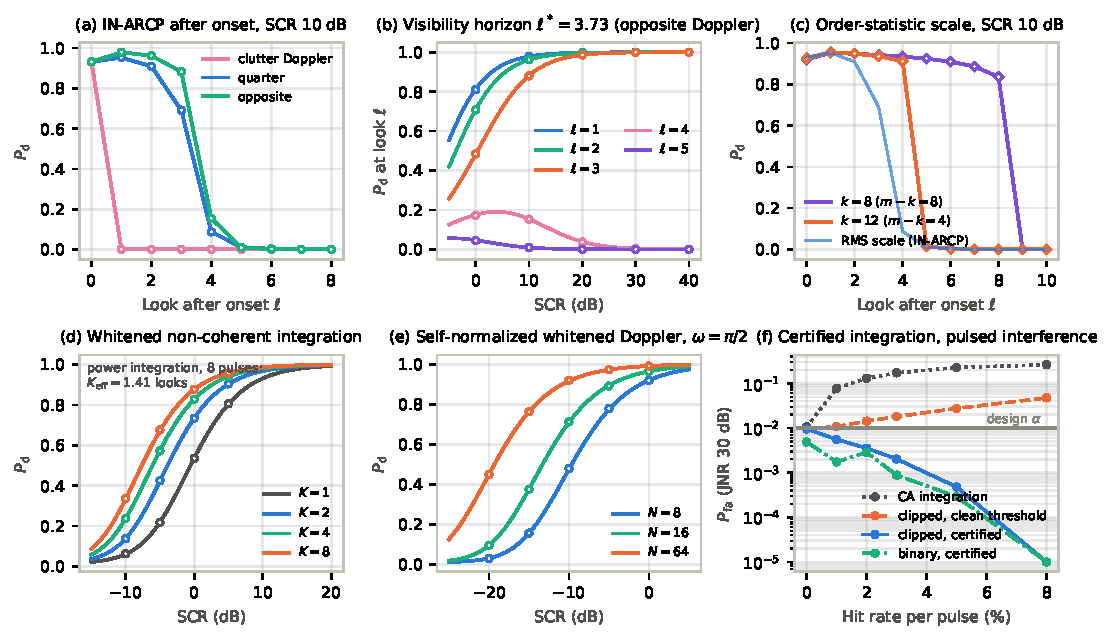
\includegraphics[width=\textwidth]{fig_theory.pdf}
\caption{Closed forms (lines) against Monte Carlo (markers; $10^5$ episodes per point), AR(1) compound-Gaussian clutter with $\rho=0.93e^{-0.2\mathrm j}$, lognormal texture, $m=16$, $P_{\rm fa}=0.01$. (a) Proposition~\ref{prop:rank1} after onset; (b) the visibility horizon of Corollary~\ref{cor:horizon}; (c) order-statistic scales, exact law by quadrature; (d) integration law \eqref{eq:dwellpd}; (e) P-ANMF with unknown Doppler; (f) Theorem~\ref{thm:cert}: false-alarm probability under pulsed interference (30~dB, Gaussian amplitudes) against the hit rate.}
\label{fig:theory}
\end{figure*}


\section{Experimental Design}\label{sec:design}
\emph{IPIX sea clutter.} The 14 openly available IPIX Dartmouth 1993 stare sessions \cite{ipixweb}: X-band, 1~kHz pulse repetition, 14 range cells of 15~m, six dates with wave heights of 0.8--3.8~m \cite{haykin1995,farina1997}. Preprocessing follows the providers' recipe. Target cells and one guard cell on each side are excluded from clutter; Section~\ref{sec:realtarget} uses the primary target cell. The two like-polarized channels are analysed separately. Each session is split into thirds with 2,000-pulse gaps; rotations 2 and 3 of (train, calibrate, test) give \NUnitsConf{} evaluation units. Rotation~1 was used during development, so the rotations are a frozen-protocol evaluation on the development campaign, not an untouched confirmation. Day transfer and a two-series hold-out are in the Supplementary Material.

\emph{77~GHz FMCW data.} The open JKU parking-lot dataset \cite{jku2026}: 76--77~GHz chirp sequences (34~$\mu$s chirp period, 128 chirps per frame, 100 frames), a static scene of parked cars, a clean reference run, and runs with an unsynchronized interferer, dense (scenario A, \JHitA\% of chirps hit) and sparse (scenario C, \JHitC\%). Range bins 8--247 of receivers 0, 5, 10, 15 of both stations are used.

\emph{Protocols.} Every study had its methods, hyperparameters, metrics and stated expectations frozen, and the protocol file hashed, before any outcome was computed: the main IPIX study (R7), onset detection (R8), the baselines and persistent targets (R9), classical detectors and gradual emergence (R10), order-statistic normalization and real interference (R11), and low-$P_{\rm fa}$ calibration, ANMF baselines, the real target and pulsed interference (R12). The freezes are hash-recorded in the code repository, not with an external registry; later analyses are labelled exploratory. In R12, \RTwelveMet{} of \RTwelveAll{} expectations were met.

\emph{Detectors and thresholds.} Per-look scores use $m=16$; dwell detectors use a 16-pulse history and an 8-pulse dwell, the median as OS history scale, clip level $c=6$ and binary threshold $\eta=6$. The ANMF uses the 8-pulse dwell and secondary vectors from the clutter cells at least two cells away, at five time positions (20--35 vectors), with the sample covariance or the Tyler estimator \cite{pascal2008fp}. Power detectors normalize by the same 16 history samples (CA16) or by the cell's power over $\pm1024$ pulses (CAloc). Conformal thresholds are calibrated on clean calibration-third episodes, non-overlapping for the low-$P_{\rm fa}$ study (about 23,000 per unit). Model-based rules are the laws of Sections~\ref{sec:onsetlaws}--\ref{sec:laws} at the fitted model, Gaussian plug-ins, the Kraut--Scharf and fixed-point ANMF laws, Gaussian simulation, and an AR residual bootstrap of the sieve type \cite{qu2024sieve}.

\emph{Targets and interference.} Swerling-1 targets are injected at SCRs from $-5$ to 25~dB relative to the local power: in the predicted pulse (onset), persistent from a given pulse with random Doppler, or rising linearly over $L$ pulses. Pulsed interference is injected into IPIX test segments and secondary data: each pulse is hit independently with probability $p\in\{0.02,0.05\}$, with complex Gaussian amplitude of 10 or 30~dB relative to the local power. On the 77~GHz data targets are injected in the raw ADC domain as beat tones and pass through the same processing. Intervals are 95\% day-cluster bootstrap intervals (six days, 10,000 resamples).

\section{Results}
\subsection{False-alarm control across clutter power and down to $10^{-4}$}\label{sec:fa}
\begin{table}[!t]
\centering\footnotesize
\caption{Measured false-alarm rate / design $\alpha$ on IPIX test thirds (\NUnitsConf{} units, pooled). Conformal: split-conformal threshold. Model-based: the rule in parentheses at the fitted model. Bold: outside $[0.5,2]$.}
\label{tab:lowpfa}
\setlength{\tabcolsep}{2.2pt}
\begin{tabular}{lcccccc}
\toprule
 & \multicolumn{3}{c}{Conformal} & \multicolumn{3}{c}{Model-based rule}\\
\cmidrule(lr){2-4}\cmidrule(lr){5-7}
$\alpha$ & $10^{-2}$ & $10^{-3}$ & $10^{-4}$ & $10^{-2}$ & $10^{-3}$ & $10^{-4}$\\
\midrule
\emph{Per look} &&&&&&\\
IN-ARCP (CA law) & 1.01 & 1.03 & 0.73 & 0.96 & 1.02 & 1.92\\
\quad residual bootstrap &  &  &  & 1.63 & \textbf{2.43} & \textbf{4.27}\\
IN-AR(4) (CA law) & 1.00 & 1.02 & 0.86 & 1.03 & 1.19 & \textbf{2.73}\\
OS scale, $k=8$ (OS law) & 1.04 & 1.02 & 0.92 & \textbf{2.15} & \textbf{8.34} & \textbf{45.9}\\
NA-AR(4) (Gaussian) & 1.00 & 1.05 & 1.04 & 1.56 & \textbf{2.79} & \textbf{7.46}\\
Power, CA (white law) & 1.00 & 1.00 & 0.75 & 0.80 & 0.56 & \textbf{0.49}\\
Power, OS (white law) & 1.01 & 0.98 & 0.75 & \textbf{2.07} & \textbf{5.56} & \textbf{18.3}\\
\emph{Eight-pulse dwell} &&&&&&\\
Integration (law \eqref{eq:dwellpfa}) & 1.02 & 1.05 & 1.02 & \textbf{2.02} & \textbf{4.35} & \textbf{14.3}\\
PAMF-H, one Doppler (CA law) & 0.99 & 1.00 & 0.89 & 1.97 & \textbf{3.66} & \textbf{9.88}\\
P-ANMF, one bin (Beta) & 1.10 & 1.14 & 1.10 & 1.78 & \textbf{3.05} & \textbf{5.47}\\
P-ANMF, max (Fisher's $g$) & 1.04 & 1.04 & 1.47 & \textbf{4.36} & \textbf{13.1} & \textbf{49.6}\\
ANMF-SCM (Kraut--Scharf) & 1.06 & 1.04 & 0.85 & \textbf{2.02} & \textbf{3.57} & \textbf{8.07}\\
ANMF-Tyler (FP law) & 1.04 & 1.05 & 0.82 & 1.62 & \textbf{2.66} & \textbf{6.01}\\
Clipped, OS scale (Gaussian sim.) & 1.05 & 0.67 & \textbf{0.03} & \textbf{4.84} & \textbf{17.2} & \textbf{59.9}\\
\bottomrule
\end{tabular}

\end{table}
Table~\ref{tab:lowpfa} is the central calibration result. The conformal thresholds hold every statistic within \LConfMinThree--\LConfMaxThree{} times design at $10^{-3}$ and \LConfMinFour--\LConfMaxFour{} times at $10^{-4}$, except the clipped integrator, which is conservative (\LClipConfThree{} and \LClipConfFour) because its statistic saturates at $Kc$; at $10^{-4}$ each unit contributes about two false alarms, so the per-statistic intervals are wide. The model-based rules fail in the tail: at $10^{-4}$ the Gaussian laws of the whitened dwell and Doppler statistics exceed design \LDinFour-fold (integration), \LPamfFour-fold (PAMF), \LPanmfFour-fold (P-ANMF with Fisher's $g$) and \LClipGFour-fold (clipped integration), the OS law \LOsFour-fold and the NA Gaussian plug-in \LNaFour-fold. The ANMF laws fail as well, \LScmThree{} (sample covariance) and \LFpThree{} (Tyler) times design at $10^{-3}$, and a residual bootstrap that resamples real innovations still exceeds design \LBootFour-fold at $10^{-4}$, consistent with dependence among the innovations of an episode that independent resampling discards. The white-noise laws of the power detectors are off in both directions. The CA law of the IN-ARCP score is the most robust model-based rule (\LInAnalThree{} at $10^{-3}$, \LInAnalFour{} at $10^{-4}$), plausibly because its scale averages all 16 history innovations. The failures are largest for statistics built on order statistics, few innovations or a self-normalizing dwell, consistent with real innovations having heavier tails than the Gaussian model.

Across clutter power, the conformal false-alarm rate of IN-ARCP at a design of 0.01 ranges from \QPfaINMin{} to \QPfaINMax{} across texture quintiles (a factor of \QPfaINSpread, and \LInConfSpreadThree{} at $10^{-3}$), against a factor of \QPfaUSpread{} for conformal prediction without innovation normalization, \QPfaRMSSpread{} for raw-RMS normalization and \QPfaMLPSpread{} for an invariant neural centre. Amplitude equivariance alone therefore does not keep a score pivotal on real clutter; innovation normalization does. The texture-conditional coverage curves, the noise-aware disc widths (\SameNAFourA{} times the innovation-normalized AR(4) radius [\SameLoNAFourA, \SameHiNAFourA] within sessions, gains that largely vanish across days) and the exact law's prediction of cross-day coverage (mean absolute error \CFiveMaeA) are in the Supplementary Material.

\subsection{Detection of new returns}\label{sec:detect}
\begin{figure}[!t]
\centering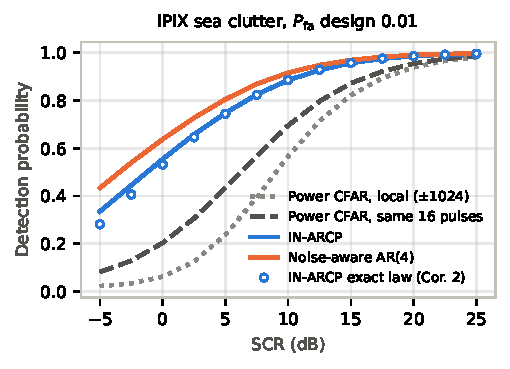
\includegraphics[width=\columnwidth]{fig_detection_col.pdf}
\caption{Onset detection on IPIX (\DetNTest{} test episodes, $P_{\rm fa}=0.01$): Swerling-1 targets in the predicted sample. Circles: exact law of Corollary~\ref{cor:detect} with the clutter+noise model fitted on each unit's training third.}
\label{fig:detect}
\end{figure}
For a target that appears in the predicted pulse (Fig.~\ref{fig:detect}), IN-ARCP needs \DetINGainCAHalf~dB [\DetINGainCALoHalf, \DetINGainCAHiHalf] less SCR than power detection on the same pulses and \DetINGainLocHalf~dB less than the long-window power detector at $P_{\rm d}=0.5$, with a day-to-day range of \DayGainMin--\DayGainMax~dB. The exact law predicts $P_{\rm d}$ with a mean absolute error of \DetMae{} per unit and SCR, and accounts for the gain being below the clutter-only whitening factor (\DetNaiveGain~dB) through thermal noise (Proposition~\ref{prop:gain}). The Gaussian threshold of IN-ARCP attains the same sensitivity at a similar false-alarm rate: the gain is whitening, not calibration.

\begin{table}[!t]
\centering\footnotesize
\caption{SCR (dB) for $P_{\rm d}=0.5$ and $0.9$ over an 8-pulse dwell, persistent Swerling-1 target with random Doppler from the first dwell pulse (IPIX, conformal thresholds). $\le-5$: reached at the lowest SCR tested; n.r.: not reached at 25~dB.}
\label{tab:dwell}
\setlength{\tabcolsep}{4pt}
\begin{tabular}{lccc}
\toprule
 & \multicolumn{2}{c}{$\alpha=0.01$} & $0.001$\\
\cmidrule(lr){2-3}
 Detector & $P_{\rm d}=0.5$ & $0.9$ & $0.5$\\
\midrule
PAMF-H & $\le-5$ & 5.1 & -4.3\\
Integration, AR(4) & $\le-5$ & 7.0 & -1.6\\
Integration, AR(1) & -4.4 & 8.3 & -0.1\\
Clipped, OS scale & -2.3 & 13.0 & n.r.\\
Binary, OS scale & -1.2 & 14.5 & n.r.\\
ANMF-SCM & -0.2 & 20.3 & 9.5\\
ANMF-Tyler & 0.4 & 20.3 & 9.8\\
P-ANMF & 0.2 & n.r. & n.r.\\
IN-ARCP, first look & -1.2 & 11.0 & 1.9\\
Power OS, first look & 9.4 & 19.5 & 14.3\\
\bottomrule
\end{tabular}

\end{table}
\label{sec:classical}Over an 8-pulse dwell (Table~\ref{tab:dwell}), the history-normalized coherent PAMF is the most sensitive detector, and AR non-coherent integration of the innovations is close to it. With one dwell pulse the PAMF and the AR(4) score give identical decisions. The ANMF needs at least \AFpMinusPamf~dB [\AFpMinusPamfLo, \AFpMinusPamfHi] more SCR than the PAMF (Tyler estimator), plausibly because 20--35 secondary vectors from neighbouring cells estimate an 8-dimensional covariance less well than a four-coefficient AR model fitted on training data does, and the P-ANMF pays for normalizing by a dwell that contains the target. The clipped and binary integrators cost \AClipMinusDin~dB [\AClipMinusDinLo, \AClipMinusDinHi] against plain integration at $\alpha=0.01$ (the protocol expected at most 1.5~dB), and at $10^{-3}$ the clip level $c=6$ saturates them; the clip level must scale with the per-look threshold at the design $\alpha$. The power OS detector on the cell's own history (clutter-map OS-CFAR) needs \AOsrawMinusIn~dB [\AOsrawMinusInLo, \AOsrawMinusInHi] more SCR than IN-ARCP at the first look: the sensitivity comes from whitening, not from the order statistic. A Hann-windowed 8-pulse Doppler filter bank with range CA normalization needs \ClINvsMTD~dB more SCR than integrated IN-ARCP, and all whitening detectors lose sensitivity for targets at the clutter Doppler (PAMF by \ClPAMFMatched~dB).

Gradual emergence limits every history-normalized detector. When the target amplitude rises over $L$ pulses before the first look, IN-ARCP's first-look gain over power detection falls from \RampGainOne~dB (abrupt) to \RampGainEight~dB ($L=8$), and at $L=16$ it is barely detected ($P_{\rm d}=\RampPdSixteen$ at 10~dB), whereas the PAMF over the dwell loses only \RampPAMFLoss~dB; the exact law reproduces the ramps (mean absolute error \RampMae).

\subsection{After the onset}\label{sec:onset}
\begin{figure}[!t]
\centering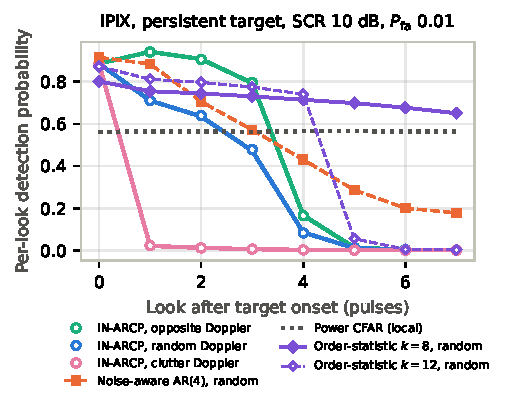
\includegraphics[width=\columnwidth]{fig_onset_col.pdf}
\caption{Per-look detection probability after the onset of a persistent Swerling-1 target on IPIX (SCR 10~dB, per-look $P_{\rm fa}$ 0.01). Markers: measured; lines: exact law with the onset signature at the fitted model (exploratory). Purple: OS scores.}
\label{fig:onset}
\end{figure}
A target that appears usually stays. As the rank-one law predicts, IN-ARCP loses a persistent target as it enters the history (Fig.~\ref{fig:onset}): at 10~dB its per-look $P_{\rm d}$ falls from \OnLookZero{} to \OnLookFour{} over five looks, a target at the clutter Doppler is lost after one look (\OnMatchedOne) and one at the opposite Doppler survives several (\OnOppOne{} at the second look), in line with the visibility horizon of \ThHorizonOpp{} looks in Corollary~\ref{cor:horizon}. The exact law with the onset signature reproduces these decays with mean absolute errors of \OnTheoryMaeRand, \OnTheoryMaeMatch{} and \OnTheoryMaeOpp{} for random, clutter and opposite Doppler. The median OS score keeps the target at \OsPersFirst--\OsPersLast{} over all eight looks at a cost of \OsCostEight~dB, and each OS variant fails exactly at the first look where the target occupies more than $m-k$ history innovations, as \eqref{eq:osstrong} states.

\subsection{The real IPIX target}\label{sec:realtarget}
\begin{table}[!t]
\centering\footnotesize
\caption{Real IPIX target (primary cell, test thirds, \NUnitsConf{} units): mean $P_{\rm d}$ at design $P_{\rm fa}=10^{-3}$ versus dwell $N$; in parentheses, measured clutter $P_{\rm fa}$ ($\times10^{-3}$). P-ANMF with Fisher's $g$ uses the analytic threshold.}
\label{tab:target}
\setlength{\tabcolsep}{4pt}
\begin{tabular}{rcccc}
\toprule
 & \multicolumn{2}{c}{P-ANMF} & Range CA & ANMF\\
\cmidrule(lr){2-3}
$N$ & conformal & Fisher's $g$ & integration & Tyler\\
\midrule
8 & 0.22 (1.1) & 0.37 (13) & 0.003 & 0.13\\
16 & 0.22 (1.3) & 0.45 (32) & 0.003 & 0.18\\
32 & 0.22 (1.3) & 0.56 (69) & 0.004 & --\\
64 & 0.30 (1.3) & 0.67 (121) & 0.004 & --\\
128 & 0.37 (1.2) & 0.75 (178) & 0.004 & --\\
256 & 0.40 (1.5) & 0.79 (235) & 0.004 & --\\
512 & 0.37 (2.0) & 0.83 (299) & 0.005 & --\\
1024 & 0.41 (2.6) & 0.87 (404) & 0.007 & --\\
\bottomrule
\end{tabular}

\end{table}
The IPIX reference target is present throughout each recording. Proposition~\ref{prop:blind} predicts that history-normalized detectors cannot see it, and on the real data they do not: IN-ARCP and the clipped integrator exceed their thresholds on the target cell at a rate of 0.0004, below their clutter false-alarm rates. Self-normalized whitened Doppler detects it (Table~\ref{tab:target}): $P_{\rm d}=\TPanmfEight$ over 8 pulses, rising to \TPanmfTwoFiveSix{} over 256 and \TPanmfThousand{} over 1,024 pulses at a calibrated false-alarm rate. Its analytic Fisher's $g$ threshold is unusable on real clutter (measured $P_{\rm fa}$ \TFisherPfaEight{} at $N=8$ and \TFisherPfaThousand{} at $N=1024$), because a four-coefficient AR model fitted on neighbouring cells does not whiten long dwells. Range CA integration and the ANMF barely detect this target. These detection probabilities are far below those reported by long-observation learned detectors (0.91 at $10^{-3}$ with 1.024~s \cite{qu2023sensors}), which use different statistics and evaluation; P-ANMF is a short-dwell detector whose value here is a calibrated threshold, not sensitivity.

\subsection{Pulsed interference}\label{sec:interf}
\begin{table}[!t]
\centering\footnotesize
\caption{Pulsed interference at $\alpha=0.01$: measured $P_{\rm fa}/\alpha$ and SCR (dB) for $P_{\rm d}=0.5$. IPIX: injected, 30~dB, hit probability $p$ per pulse. 77~GHz run C: real interference, 4.6\% of chirps hit, no fast-time mitigation. Bold: $P_{\rm fa}/\alpha>1.5$.}
\label{tab:interf}
\setlength{\tabcolsep}{2.4pt}
\begin{tabular}{lcccccc}
\toprule
 & \multicolumn{2}{c}{IPIX, $p=2\%$} & \multicolumn{2}{c}{IPIX, $p=5\%$} & \multicolumn{2}{c}{77 GHz, run C}\\
\cmidrule(lr){2-3}\cmidrule(lr){4-5}\cmidrule(lr){6-7}
 Detector & $P_{\rm fa}/\alpha$ & SCR$_{50}$ & $P_{\rm fa}/\alpha$ & SCR$_{50}$ & $P_{\rm fa}/\alpha$ & SCR$_{50}$\\
\midrule
Integration, AR(1) & \textbf{12.9} & -1.5 & \textbf{21.2} & 11.0 & 1.42 & 7.1\\
PAMF-H & \textbf{13.7} & $\le-5$ & \textbf{22.1} & 4.3 & -- & --\\
P-ANMF & 0.82 & 5.7 & 0.55 & 18.6 & -- & --\\
ANMF-Tyler & 1.07 & 3.4 & 1.21 & 9.0 & -- & --\\
Clipped, clean threshold & 1.07 & -2.2 & 1.28 & -2.1 & 1.29 & 8.1\\
Clipped, certified & 0.55 & -0.9 & 0.11 & 7.1 & 0.54 & 14.5\\
Binary, certified & 0.32 & 0.2 & 0.05 & 8.2 & 0.33 & 15.8\\
\bottomrule
\end{tabular}

\end{table}
With injected pulsed interference on IPIX (Table~\ref{tab:interf}), non-coherent integration and the PAMF exceed their design false-alarm probability \IPfaMinAll- to \IPfaMaxAll-fold across the four conditions: a hit dwell pulse is an outlier the history does not predict. Self-normalized detectors (P-ANMF, ANMF) keep their false-alarm rate but lose sensitivity, and clipping with a clean threshold exceeds design only mildly (\IClipPfaTwo{} and \IClipPfaFive{} times). The certified clipped and binary integrators stay below design in every condition (upper interval bound at most \ICertUpperMax{} times design), as Theorem~\ref{thm:cert} guarantees; the certified clipped integrator costs \ICertCostTwo~dB at a 2\% hit rate and \ICertCostFive~dB at 5\%.

On the 77~GHz data the interference is real and chirp-wide. In the sparse run the certified clipped integrator holds the false-alarm rate at \JCertPfaC{} times design without any fast-time mitigation (\JCertPfaCZ{} with zeroing), while non-coherent integration runs at \JDinPfaC{} times design overall and \JDinPfaCone{} times in segments with one or two hit chirps. The certificate costs about 3~dB on hit-free segments (SCR \JCertScrCclean{} against \JClipScrCclean~dB) and more overall. In the dense run, where 45\% of chirps are hit, real interference mainly masks targets rather than raising false alarms (non-coherent integration \JDinPfaA{} times design), and certification is nearly vacuous. Fast-time zeroing restores the design false-alarm rate for every detector (\JZPfaC{} for integration in run C) at a small sensitivity cost, and AR reconstruction of the zeroed samples adds only \JZarGainA~dB. Where interference can be excised in fast time, excision is the better tool; certification is the guarantee when it cannot, as for pulsed radars whose interference occupies whole pulses.

\subsection{Thermal noise on the second radar}\label{sec:jku}
The parking-lot scene spans CNRs from below $-5$ to about 20~dB. IN-ARCP coverage rises from \JInLow{} in noise-dominated cells to \JInHigh{} at 10--20~dB CNR, and the exact law of Corollary~\ref{cor:texture} predicts the class coverages with mean absolute error \JMae. On the false-alarm scale the invariance is lost in the direction the law predicts (\JPfaRatioLow{} to \JPfaRatioHigh{} times design across CNR classes) but not in size. The gain over local power detection follows the sign of Proposition~\ref{prop:gain}: a loss of \JINGainLow~dB in noise-dominated cells and a gain of \JINGainHigh~dB at 10--20~dB CNR; the NA score avoids most of the low-CNR loss (Supplementary Material).

\section{Discussion}
\subsection{Design rules}
The laws and measurements combine into a short recipe for a cell-wise detector in correlated clutter.
\begin{enumerate}[leftmargin=*,itemsep=1pt]
\item Whiten each cell with an AR model fitted on clutter training data; use the RMS innovation scale (the most robust in the tail) or an OS scale when targets may persist for up to $m-k$ looks.
\item Set thresholds conformally on clean clutter episodes. The calibration size follows from the Beta law: about $16/\alpha$ episodes keep the false-alarm probability below $2\alpha$ with probability 0.95. Do not trust Gaussian-model tails below $10^{-2}$ on real sea clutter.
\item Predict sensitivity with Table~\ref{tab:laws} at the whitened SCR $S\,P/S_c(\omega)$; the visibility horizon \eqref{eq:horizon} tells how long a history-normalized screen keeps a target.
\item For targets that persist through the history, use a self-normalized whitened Doppler statistic or reference-cell normalization; for targets that may emerge gradually, a coherent dwell detector (PAMF).
\item Under pulsed interference that cannot be excised in fast time, integrate clipped normalized innovations with a certified threshold, choosing the clip level for the design $\alpha$; with a bound on the hit rate the false-alarm probability holds for any interference power.
\end{enumerate}

\subsection{Limitations}
\begin{itemize}[leftmargin=*,itemsep=1pt]
\item \textbf{Data.} The sea-clutter evidence comes from one radar and one campaign, and the IPIX rotations reuse recordings seen during development. A second sea-clutter database \cite{dewind2010csir} is needed to establish generality.
\item \textbf{Targets.} Detection results use injected targets, except the real IPIX target, on which only self-normalized Doppler detects, with modest probability. Gradually emerging targets defeat per-look screening.
\item \textbf{Laws.} The closed forms assume the true AR model and pure compound-Gaussian clutter; on real clutter they predict detection closely, but real clutter departs from the model in the far tail, so model-based thresholds fail there and calibration is needed.
\item \textbf{Certification.} The certificate needs the hit positions to be independent of the clutter and dominated by the hit model; interference below the hit detector counts as clutter. Its cost grows quickly with the hit rate, and at a 45\% hit rate it is nearly vacuous.
\item \textbf{Calibration.} Conformal validity is marginal and requires exchangeable calibration and test episodes; across days the noise-aware gains vanish and online recalibration is vulnerable to target contamination \cite{gibbs2021aci,wang2026corrupted} (Supplementary Material).
\end{itemize}

\section{Conclusion}
Whitening a range cell with an autoregressive model and normalizing by its own innovation power turns correlated compound-Gaussian clutter into the independent exponential samples on which classical CFAR theory is built. The laws then return with the SCR multiplied by the whitening factor, and the view adds new ones: a closed-form law after target onset with a visibility horizon, its order-statistic counterpart, and a certificate for clipped integration under pulsed interference of any power. On real sea clutter the laws predict detection, the model-based thresholds fail in the tail, and conformal calibration holds the false-alarm rate to $10^{-4}$. Persistent targets need self-normalization, and gradually emerging ones a coherent dwell. Under pulsed interference the certificate holds on sea clutter and on real FMCW interference, at a cost that fast-time excision avoids when it is possible. An untouched second sea-clutter database and real-target campaigns remain the next tests.

\appendices
\section{Proof of Proposition~\ref{prop:law}}\label{app:law}
Write $X=\Sigma^{1/2}\xi$ with $\xi\sim\mathcal{CN}(0,I)$. The event is $\{X^{\mathsf H}M_qX\le0\}$ and $X^{\mathsf H}M_qX=\sum_k\lambda_kE_k$ with independent standard exponentials $E_k$. $M_q$ is positive in the direction $e_{m+1}$ and $M_q+\frac{q^2}{m}\operatorname{diag}(Q,0)$ has rank one, so by Weyl's inequality $M_q$ has exactly one positive eigenvalue; by Sylvester's law of inertia so does $\Sigma^{1/2}M_q\Sigma^{1/2}$. Partial fractions of the characteristic function $\prod_k(1-\mathrm it\lambda_k)^{-1}$ give the density of the form \cite{alnaffouri2016}; integrating over $x>0$ leaves only the term of $\lambda_+$, which is \eqref{eq:exactlaw}.

\section{Proofs of Corollary~\ref{cor:detect}, Propositions~\ref{prop:blind} and~\ref{prop:rank1}, and Theorem~\ref{thm:cert}}\label{app:detect}
\emph{Corollary~\ref{cor:detect}.} A Swerling-1 target makes the episode $\mathcal{CN}(0,\Sigma+SP\,vv^{\mathsf H})$. At $r=\rho$ in pure AR(1) clutter, $Y-\rho H_m=E+A$ with independent $E\sim\mathcal{CN}(0,\sigma^2(1-|\rho|^2))$ and $A\sim\mathcal{CN}(0,S\sigma^2)$, and $ms_\rho^2/(\sigma^2(1-|\rho|^2))$ is a sum of $m$ unit exponentials, which gives \eqref{eq:pdclosed} as a Gamma moment-generating function.

\emph{Proposition~\ref{prop:blind}.} The score is homogeneous of degree zero, so its value at $\sigma Z+Au$ equals that at $\sigma Z/A+u$ and tends to its value at $u$; at $u$ the numerator is $|1-re^{-\mathrm j\omega}|$ and $ms_r(u)^2=(1-|r|^2)+(m-1)|1-re^{-\mathrm j\omega}|^2$. Dominated convergence gives $P_{\rm d}\to0$.

\emph{Proposition~\ref{prop:rank1}.} In whitened units the episode is $\mathcal{CN}(0,I+uu^{\mathsf H})$ and the event is $x^{\mathsf H}Mx>0$, $M=\operatorname{diag}(-\beta I_m,1)$. The eigenvalues of $M(I+uu^{\mathsf H})$ are $-\beta$ ($m-1$ times) and the roots of $(\lambda-1)(\lambda+\beta)-a(\lambda+\beta)+\beta b(\lambda-1)=0$ (rank-one update of a diagonal matrix). With $\lambda_+>0>\lambda_-$, $\PP\{\lambda_+E_+>|\lambda_-|E_-+\beta\Gamma_{m-1}\}$ is \eqref{eq:rank1}. For the horizon, $\lambda_+\to\infty$ or stays bounded as $S\to\infty$ according to the sign of $|d|^2-\beta\{1+(\ell-1)|d|^2\}$.

\emph{Theorem~\ref{thm:cert}.} The $k_H$-th smallest history power is nondecreasing in each power, so over all values of the corrupted entries it is at least its value with those entries at zero; uncorrupted dwell terms are clean powers over a scale at least that large, and corrupted clipped terms are at most $c$. Hence $T\le W(x,\mathcal H)$, and $W$ is nondecreasing in $\mathcal H$. If $\mathcal H\subseteq\tilde{\mathcal H}\sim Q$ (a coupling under stochastic dominance) with $\tilde{\mathcal H}$ independent of the clutter, then $T\le W(X,\tilde{\mathcal H})$, and $(X_i,\mathcal H_i)$ and $(X,\tilde{\mathcal H})$ are exchangeable, so the split-conformal rank argument bounds $\PP\{T>\widehat q\}$ by $\alpha$. Details, the order-statistic and integration laws, and the Fisher's $g$ detection law are in the Supplementary Material.

\section*{Code and Data Availability}
Code, the frozen protocols with their hashes, outcome hashes, analysis outputs and figure scripts are in the project repository, https://github.com/razaumair2203-ux/inarcp, release \textbf{[AUTHORS: insert tag and commit after pushing branch research/r7-clutter]}; the Python package \texttt{inarcp} (version 0.3.0) implements the detectors and laws. The IPIX data are available from McMaster University \cite{ipixweb} and the 77~GHz data from Zenodo \cite{jku2026}.

\section*{Acknowledgment}
The authors acknowledge the McMaster University IPIX radar group and L.~Rienessl and R.~Feger (Johannes Kepler University Linz) for making their radar data openly available. Generative AI tools were used in this work. OpenAI Codex assisted earlier versions with manuscript editing, literature organization, and implementation and verification code. Anthropic Claude assisted with literature checks, derivations and their numerical verification, implementation, the design and execution of the real-data and synthetic studies, and drafting of all sections. \textbf{[AUTHORS: replace this bracket with a statement of which derivations, analyses and text the authors independently verified.]} The authors take full responsibility for the content.

\bibliographystyle{IEEEtran}
\bibliography{references}

\end{document}
